\documentclass[a4paper, reqno, twoside]{amsart}

\usepackage{amsmath}
\usepackage{amssymb}
\usepackage{graphicx}
\usepackage{enumerate}
\usepackage[all]{xy}
\usepackage{tikz}
\usetikzlibrary{arrows,decorations.pathmorphing,backgrounds,positioning,fit,petri,decorations.pathreplacing}

\usepackage{hyperref}
\usepackage{comment}
\usepackage{xspace}
\usepackage{mathtools}

\hypersetup{pdftitle={Normal complex surface singularities with rational homology disk smoothings},pdfauthor={Heesang Park, Dongsoo Shin, Andr\'as I. Stipsicz},pdfkeywords={complex surface singularity, Milnor fiber,
rational homology disk, weighted homogeneous singularity},}

\newtheorem{theorem}{Theorem}[section]
\newtheorem{lemma}[theorem]{Lemma}
\newtheorem{proposition}[theorem]{Proposition}
\newtheorem{corollary}[theorem]{Corollary}
\newtheorem{maintheorem}[theorem]{Main Theorem}

\theoremstyle{definition}

\newtheorem{definition}[theorem]{Definition}
\newtheorem{remark}[theorem]{Remark}
\newtheorem{note}[theorem]{Note}
\newtheorem{example}[theorem]{Example}
\newtheorem{notation}[theorem]{Notation}

\numberwithin{equation}{section}

\begin{document}

\title[Singularities with rational homology disk smoothings]{Normal complex surface singularities with rational homology disk smoothings}

\author[H. Park]{Heesang Park}

\address{Department of Mathematics, Konkuk University, Seoul 143-701, Korea}

\email{HeesangPark@konkuk.ac.kr}

\author[D. Shin]{Dongsoo Shin}

\address{Department of Mathematics, Chungnam National University,
  Daejeon 305-764, Korea}

\email{dsshin@cnu.ac.kr}

\author[A. I. Stipsicz]{Andr\'{a}s I. Stipsicz}

\address{R\'enyi Institute of Mathematics, Re\'altanoda utca 13-15.,
Budapest 1053, Hungary}

\email{stipsicz@renyi.hu}

\subjclass[2000]{14B07, 14J17, 32S30}

\keywords{surface singularity, Milnor fiber, rational homology disk smoothing}

\begin{abstract}
We show that if the minimal good resolution graph of a normal surface
singularity contains at least two nodes (i.e.\  vertex with valency at
least 3) then the singularity does not admit a smoothing with Milnor
fiber having rational homology equal to the rational homology of the
4-disk $D^4$ (called a rational homology disk smoothing).  Combining
with earlier results, this theorem then provides a complete
classification of resolution graphs of normal surface singularities
with a rational homology disk smoothing, verifying a conjecture of
J. Wahl regarding such singularities.  Indeed, together with a recent
result of J. Fowler we get the complete list of normal surface
singularities which admit rational homology disk smoothings.
\end{abstract}

\maketitle

\section{Introduction}
\label{sec:intro}
Let $(X, 0)$ be a (germ of a) normal complex surface singularity. A \emph{smoothing} of $(X, 0)$ is a flat surjective map $\pi\colon (\mathcal{X}, 0) \to (\Delta, 0)$, where $(\mathcal{X}, 0)$ has an
isolated 3-dimensional singularity and $\Delta = \{t \in \mathbb{C}
\mid {\ensuremath \left\lvert {t} \right\rvert} < \epsilon \}$, such that $(\pi^{-1}(0), 0)$ is
isomorphic to $(X, 0)$ and $\pi^{-1}(t)$ is smooth for every $t \in
\Delta \setminus \{0\}$. Assume that $(X,0)$ is embedded in $(\mathbb{C}^N,
0)$. Then there exists an embedding of $(\mathcal{X}, 0)$ in
$(\mathbb{C}^N \times \Delta, 0)$ such that the map $\pi$ is induced
by the projection $\mathbb{C}^N \times \Delta \to \Delta$ to the
second factor. The \emph{Milnor fiber} $M$ of a smoothing $\pi$ of
$(X,0)$ is defined by the intersection of a fiber $\pi^{-1}(t)$ ($t
\neq 0$) near the origin with a small ball about the origin, that
is, $M = \pi^{-1}(t) \cap B_{\delta}(0)$ ($0 < {\ensuremath \left\lvert {t} \right\rvert} \ll \delta \ll
\epsilon$).

According to the general theory of Milnor fibrations (see
Looijenga~\cite{Looijenga-1984}), $M$ is a compact 4-manifold, with the
\emph{link} $L$ of the singularity $(X,0)$ as its boundary. In particular, the
diffeomorphism type of $M$ depends only on the smoothing $\pi$; hence, the
topological invariants of $M$ are invariants of the smoothing $\pi$.  The
4-manifold $M$ has the homotopy type of a two-dimensional CW complex, thus we
have $H_i(M, \mathbb{Z})=0$ for $i > 2$. Furthermore, by
Greuel--Steenbrink~\cite[Theorem~2]{Greuel-Steenbrink-1983}, the first Betti
number $b_1(M)$ is zero. Therefore, an important invariant of $M$ (hence, of
the smoothing $\pi$) is $H_2(M, \mathbb{Z})$, which is a finitely generated
free abelian group. The \emph{Milnor number} $\mu$ of the smoothing $\pi$ is
given by the second Betti number $\mu=\dim {H_2(M, \mathbb{Q})}$.

If $\mu=0$, that is, $H_i(M, \mathbb{Q})=H_i(D^4,\mathbb{Q})=0$ for
$i>0$, we say that $M$ is a \emph{rational homology disk} ({$\mathbb{Q}$HD\xspace} for
short).  Correspondingly, a smoothing $\pi$ with $\mu=0$ is called a
\emph{rational homology disk smoothing} (`{$\mathbb{Q}$HD smoothing\xspace}' for short). For
example, any cyclic quotient singularity of type $\frac{1}{p^2}(1,
pq-1)$ with two relatively prime integers $p>q$ admits a
{$\mathbb{Q}$HD smoothing\xspace}. Indeed, according to
Looijenga--Wahl~\cite[(5.10)]{Looijenga-Wahl-1986} and
Wahl~\cite[(5.9.1)]{Wahl-1981}, among cyclic quotient singularities
these are the only ones having a
{$\mathbb{Q}$HD smoothing\xspace}. Koll\'ar--Shepherd-Barron~\cite{Kollar-Shepherd-Barron-1988}
made substantial use of the fact that the {$\mathbb{Q}$HD smoothing\xspace} of a singularity of
type $\frac{1}{p^2}(1, pq-1)$ is a quotient of a smoothing of its
index one cover; they invented the term ``$\mathbb{Q}$-Gorenstein
smoothing''.

Singularities of type $\frac{1}{p^2}(1, pq-1)$ play an important role in the
Koll\'ar--Shepherd-Barron--Alexeev (KSBA) compactification of moduli spaces of
complex surfaces of general type. For instance,
Y.~Lee--J.~Park~\cite{Lee-Park-K^2=2} constructed a singular surface with
singularities of type $\frac{1}{p^2}(1, pq-1)$. Since the Milnor fibers of
these singularities are topologically very simple, it is easy to control
(topological) invariants of the smoothing of the singular surface. Hence, by
smoothing the singular surface, they constructed examples of complex surfaces
of general type with prescribed topological invariants. In particular, they
constructed a point lying on the boundary of the KSBA compactification of a
moduli space of complex surfaces of general type. Using similar ideas, many
important examples of complex surfaces of general type have been constructed;
see, for example, \cite{Keum-Lee-Park, PPS-K3, PPS-K4, PPS-pg1, PPS-H1Z4,
  PSU}. These constructions were
motivated by the \emph{rational blow-down} construction of
Fintushel--Stern~\cite{Fintushel-Stern-1997}, and its generalization by
J. Park~\cite{JPark-1997}:
in this smooth construction one substitutes the
tubular neighbourhood of a configuration of surfaces in a 4-manifold
intersecting each other according to the resolution graph of a singularity
with a {$\mathbb{Q}$HD smoothing\xspace} of the same singularity.
These constructions played a crucial role in
constructing exotic differentiable structures on many 4-manifolds,
cf.\  for example~\cite{Fintushel-Stern-1997, JPark-2005, PSSz, SSz}.

Therefore it is an interesting problem to classify all normal surface
singularities admitting a {$\mathbb{Q}$HD smoothing\xspace}. Such a singularity
$(X, 0)$ must be rational; in particular the resolution dual graph is
a tree and the vertices correspond to rational curves. Besides the cyclic quotient ones, further such examples were described by
Wahl~\cite{Wahl-1981}, and a list of such singularities (compiled by Wahl) was
known to the experts, cf.\  the remark on the bottom of page 505 of de Jong--van
Straten~\cite{deJong-VanStraten-1998}.

Using smooth topological ideas, in
Stipsicz--Szab\'o--Wahl~\cite{Stipsicz-Szabo-Wahl-2008} strong
necessary combinatorial conditions for the resolution graphs of
singularities with a {$\mathbb{Q}$HD smoothing\xspace} has been derived. Besides the linear graphs
(that is, the resolution graphs of cyclic quotient singularities of
type $\frac{1}{p^2}(1, pq-1)$) the potential graphs were classified
into six classes ${\ensuremath \mathcal{W}}, {\ensuremath \mathcal{M}}, {\ensuremath \mathcal{N}}$ and ${\ensuremath \mathcal{A}}, {\ensuremath \mathcal{B}},
{\ensuremath \mathcal{C}}$. In the first three classes the resolution graphs are all
star-shaped (i.e.\  each admits a unique node), with the node having
valency 3, and all these graphs are taut in the sense of
Laufer~\cite{Laufer-1973-Taut}. (Recall that a singularity is called
\emph{taut} if it is determined analytically by its resolution graph.)
The singularities corresponding to the graphs in ${\ensuremath \mathcal{W}},
{\ensuremath \mathcal{M}}$ and ${\ensuremath \mathcal{N}}$ all admit {$\mathbb{Q}$HD smoothing\xspace}.

The further three types ${\ensuremath \mathcal{A}}, {\ensuremath \mathcal{B}}$ and ${\ensuremath \mathcal{C}}$ are defined by the
following construction.  Let $\Gamma_{\ensuremath \mathcal{A}}$, $\Gamma_{\ensuremath \mathcal{B}}$,
$\Gamma_{\ensuremath \mathcal{C}}$ be the graphs given as follows.

\begin{center}
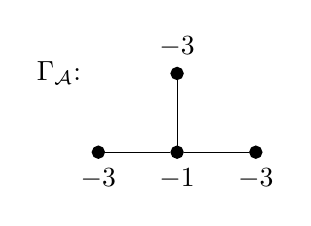
\begin{tikzpicture}
[bullet/.style={circle,draw=black!100,fill=black!100,thick,inner sep=0pt,minimum size=0.4em}]
\node[bullet] (00) at (0,0) [label=below:$-3$] {};
\node[bullet] (10) at (1,0) [label=below:$-1$] {};
\node[bullet] (11) at (1,1) [label=above:$-3$] {};
\node[bullet] (20) at (2,0) [label=below:$-3$] {};
\node (01) at (-0.5,1) {$\Gamma_{\ensuremath \mathcal{A}}$:};

\draw [-] (00) -- (10);
\draw [-] (10) -- (11);
\draw [-] (10) -- (20);
\end{tikzpicture}
\qquad
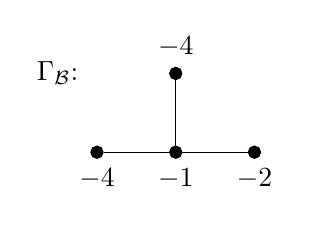
\begin{tikzpicture}
[bullet/.style={circle,draw=black!100,fill=black!100,thick,inner sep=0pt,minimum size=0.4em}]
\node[bullet] (00) at (0,0) [label=below:$-4$] {};
\node[bullet] (10) at (1,0) [label=below:$-1$] {};
\node[bullet] (11) at (1,1) [label=above:$-4$] {};
\node[bullet] (20) at (2,0) [label=below:$-2$] {};
\node (01) at (-0.5,1) {$\Gamma_{\ensuremath \mathcal{B}}$:};

\draw [-] (00) -- (10);
\draw [-] (10) -- (11);
\draw [-] (10) -- (20);
\end{tikzpicture}
\qquad
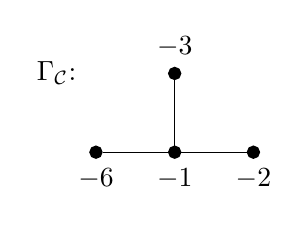
\begin{tikzpicture}
[bullet/.style={circle,draw=black!100,fill=black!100,thick,inner sep=0pt,minimum size=0.4em}]
\node[bullet] (00) at (0,0) [label=below:$-6$] {};
\node[bullet] (10) at (1,0) [label=below:$-1$] {};
\node[bullet] (11) at (1,1) [label=above:$-3$] {};
\node[bullet] (20) at (2,0) [label=below:$-2$] {};
\node (01) at (-0.5,1) {$\Gamma_{\ensuremath \mathcal{C}}$:};

\draw [-] (00) -- (10);
\draw [-] (10) -- (11);
\draw [-] (10) -- (20);
\end{tikzpicture}
\end{center}

A \emph{non-minimal graph of type ${\ensuremath \mathcal{A}}$ (or ${\ensuremath \mathcal{B}}$ or ${\ensuremath \mathcal{C}}$)}
is a graph obtained as follows: Starting with the graph
$\Gamma_{\ensuremath \mathcal{A}}$ (respectively, $\Gamma_{\ensuremath \mathcal{B}}$ or
$\Gamma_{\ensuremath \mathcal{C}}$), apply the following two \emph{blowing up
  operations}:
\begin{enumerate}
\item[(B-1)] blow up the ($-1$)-vertex\\
\begin{center}
\begin{tikzpicture}
[bullet/.style={circle,draw=black!100,fill=black!100,thick,inner sep=0pt,minimum size=0.4em}]
\node (00) at (0,0) [] {};
\node[bullet] (10) at (1,0) [label=below:$-1$] {};
\node (20) at (2,0) [] {};

\draw [dotted] (00) -- (10);
\draw [dotted] (10) -- (20);

\node (250) at (2.5,0) {};
\node (350) at (3.5,0) {};

\draw [->,decorate,decoration={snake,amplitude=.4mm,segment length=2mm,post length=1mm}] (250) -- (350);

\node (40) at (4,0) [] {};
\node[bullet] (50) at (5,0) [label=below:$-2$] {};
\node[bullet] (51) at (5,1) [label=right:$-1$] {};
\node (60) at (6,0) [] {};

\draw [dotted] (40) -- (50);
\draw [-] (50) -- (51);
\draw [dotted] (50) -- (60);
\end{tikzpicture}
\end{center}

\item[(B-2)] or blow up any edge emanating from the ($-1$)-vertex\\
\begin{center}
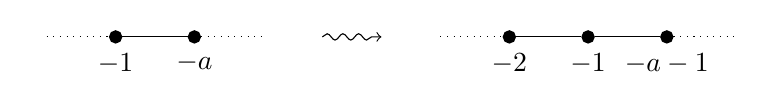
\begin{tikzpicture}
[bullet/.style={circle,draw=black!100,fill=black!100,thick,inner sep=0pt,minimum size=0.4em}]
\node (00) at (0,0) [] {};
\node[bullet] (10) at (1,0) [label=below:$-1$] {};
\node[bullet] (20) at (2,0) [label=below:$-a$] {};
\node (30) at (3,0) [] {};

\draw [dotted] (00) -- (10);
\draw [-] (10) -- (20);
\draw [dotted] (20) -- (30);

\node (350) at (3.5,0) {};
\node (450) at (4.5,0) {};

\draw [->,decorate,decoration={snake,amplitude=.4mm,segment length=2mm,post length=1mm}] (350) -- (450);

\node (50) at (5,0) [] {};
\node[bullet] (60) at (6,0) [label=below:$-2$] {};
\node[bullet] (70) at (7,0) [label=below:$-1$] {};
\node[bullet] (80) at (8,0) [label=below:$-a-1$] {};
\node (90) at (9,0) [] {};

\draw [dotted] (50) -- (60);
\draw [-] (60) -- (70);
\draw [-] (70) -- (80);
\draw [dotted] (80) -- (90);
\end{tikzpicture}
\end{center}
\end{enumerate}
and repeat these procedures of blowing up (either the new
($-1$)-vertex or an edge emanating from it) finitely many times. The
result is a non-minimal graph $\Gamma$.

A \emph{minimal graph $\overline{\Gamma}$ of type ${\ensuremath \mathcal{A}}$ (or ${\ensuremath \mathcal{B}}$ or
  ${\ensuremath \mathcal{C}}$)} corresponding to a non-minimal graph $\Gamma$ of type ${\ensuremath \mathcal{A}}$
(respectively, ${\ensuremath \mathcal{B}}$ or ${\ensuremath \mathcal{C}}$) is a graph obtained by
\begin{enumerate}
\item[(M)] \emph{modifying} the unique ($-1$)-decoration of a non-minimal
  graph $\Gamma$ of type ${\ensuremath \mathcal{A}}$ (respectively, ${\ensuremath \mathcal{B}}$ or ${\ensuremath \mathcal{C}}$) to
  ($-4$) (respectively, ($-3$) or ($-2$)).
\end{enumerate}
The classes ${\ensuremath \mathcal{A}}, {\ensuremath \mathcal{B}}$ and ${\ensuremath \mathcal{C}}$ are the collections of minimal
graphs of the respective types. It is not hard to see that a graph in
${\ensuremath \mathcal{A}}\cup {\ensuremath \mathcal{B}}\cup {\ensuremath \mathcal{C}}$ has at most one node of valency 4
(corresponding to the node of $\Gamma _{\ensuremath \mathcal{A}}, \Gamma _{\ensuremath \mathcal{B}}$ or $\Gamma
_{\ensuremath \mathcal{C}}$) and all the others are of valency 3.

Using methods of symplectic topology, in
Bhupal--Stipsicz~\cite{Bhupal-Stipsicz-2011} star-shaped graphs
admitting a {$\mathbb{Q}$HD smoothing\xspace} have been completely
classified. In particular, it has been shown that if a minimal good
resolution graph ${\overline {\Gamma}} $ is star-shaped and corresponds to a singularity with a {$\mathbb{Q}$HD smoothing\xspace}, then
${\overline {\Gamma}}$ is one of the graphs given by
Figures~\ref{fig:fig1} or~\ref{fig:fig2}.
\begin{figure}[ht]
\includegraphics[width=\textwidth]{fig1}
\caption{Star-shaped graphs with one node of degree 3 corresponding to
singularities with a {$\mathbb{Q}$HD smoothing\xspace}. We assume that $p,q,r\geq 0$.}
\label{fig:fig1}
\end{figure}

\begin{figure}[ht]
\includegraphics[scale=1]{fig2}
\caption{Star-shaped graphs with one node of degree 4 corresponding to
singularities with a {$\mathbb{Q}$HD smoothing\xspace}. The quadruple $(a,b,c;d)$ is one of
$\{ (3,3,3;4), (2,4,4;3), (2,3,6;2)\}$; furthermore $p \ge 0$.}
\label{fig:fig2}
\end{figure}

In fact, in~\cite{Wahl-2011} Wahl conjectured that the only complex
surface singularities admitting a {$\mathbb{Q}$HD smoothing\xspace} are the formerly known
examples, which are all weighted homogeneous (hence, in particular,
have resolution graphs with at most one node). In supporting this
conjecture, Wahl showed that many graphs with exactly two nodes do not
correspond to singularities with a {$\mathbb{Q}$HD smoothing\xspace},
cf.\  \cite[Theorem~8.6]{Wahl-2011}. The aim of this paper is to prove
Wahl's conjecture:

\begin{maintheorem}
\label{thm:maintheorem}
Suppose that $\overline{\Gamma}$ is a minimal negative definite graph
with at least two nodes. Then there is no complex surface singularity
with resolution graph $\overline{\Gamma}$ which admits a {$\mathbb{Q}$HD smoothing\xspace}.
\end{maintheorem}

This result, with the aforementioned result of Bhupal--Stipsicz~\cite{Bhupal-Stipsicz-2011}
provides the following classification result:

\begin{corollary}\label{cor:ClassificationOfGraphs}
  Suppose that ${\overline{\Gamma}}$ is a minimal negative definite graph with
  the property that there is a singularity which admits a {$\mathbb{Q}$HD smoothing\xspace} and has
  ${\overline{\Gamma}}$ as a resolution graph. Then ${\overline{\Gamma}}$ is
  either the linear graph corresponding to one of the cyclic quotient
  singularities of type $\frac{1}{p^2}(1,pq-1)$ (with $p>q>0$ relatively
  prime) or ${\overline{\Gamma}}$ is one of the graphs of
  Figures~\ref{fig:fig1} or~\ref{fig:fig2}. \qed
\end{corollary}

Indeed, the above result leads to the complete classification of
complex normal surface singularities with {$\mathbb{Q}$HD smoothing\xspace}.  Since the resolution
graphs of cyclic quotient singularities and the graphs of
Figure~\ref{fig:fig1} are all taut by Laufer~\cite{Laufer-1973-Taut},
for these cases the singularities themselves are determined by the
resolution graph. A graph of Figure~\ref{fig:fig2} does not determine
a unique singularity --- the analytic type depends on a complex
number, the cross ratio of the four intersection points on the
rational curve corresponding to the node of valency $4$ with its four
neighbours. According to a recent result of J. Fowler
\cite[Theorem 5(a)]{Fowler-2013}, for any graph in Figure~\ref{fig:fig2} exactly one
cross ratio determines a singularity admitting a {$\mathbb{Q}$HD\xspace} smoothing. This
value of the cross ratio is also determined by
Fowler~\cite{Fowler-2013}: it is anharmonic for $(a,b,c;d)=(3,3,3;4)$,
harmonic for $(a,b,c;d)=(2,4,4;3)$, and $9$ for
$(a,b,c;d)=(2,3,6;2)$. Therefore, as a combination of
Corollary~\ref{cor:ClassificationOfGraphs} and the result of
Fowler~\cite{Fowler-2013} we get the classification of singularities
admitting a {$\mathbb{Q}$HD smoothing\xspace}:
\begin{corollary}
  The set of complex normal surface singularities admitting a {$\mathbb{Q}$HD smoothing\xspace}
  is equal to the set of singularities we get by considering

\begin{itemize}
\item the cyclic quotient singularities of type
$\frac{1}{p^2}(1,pq-1)$ (with $p>q>0$ relatively prime),

\item the weighted homogeneous singularities corresponding to the taut graphs of
  Figure~\ref{fig:fig1}, and

\item the weighted homogeneous singularities with resolution graphs of Figure~\ref{fig:fig2},
  together with the cross ratios: anharmonic for $(a,b,c;d)=(3,3,3;4)$,
  harmonic for $(a,b,c;d)=(2,4,4;3)$, and $9$ for $(a,b,c;d)=(2,3,6;2)$. \qed
\end{itemize}
\end{corollary}

\begin{remark}
It is known that a {$\mathbb{Q}$HD smoothing\xspace} component of a cyclic quotient singularity of
type $\frac{1}{p^2}(1,pq-1)$ (with $p>q>0$ relatively prime) has
dimension one, and the {$\mathbb{Q}$HD smoothing\xspace} can always be chosen to be a
$\mathbb{Q}$-Gorenstein smoothing. In \cite{Wahl-2011, Wahl-2011-log}
Wahl verified the same properties for any weighted homogeneous surface
singularity admitting a {$\mathbb{Q}$HD smoothing\xspace}. Hence, combined with Main
Theorem~\ref{thm:maintheorem}, we conclude that any {$\mathbb{Q}$HD smoothing\xspace} of a
normal surface singularity is $\mathbb{Q}$-Gorenstein occurring over a
one-dimensional smoothing component.
\end{remark}

One of the main ideas of the proof of Theorem~\ref{thm:maintheorem} is an
extension of the result of Wahl in \cite[\S8]{Wahl-2011} about graphs
of two nodes. Let $(X, 0)$ be a germ of a rational surface
singularity, and let $\pi\colon V \to X$ be the minimal good
resolution of $X$ near $0$ with $E=\pi^{-1}(0)$ the exceptional
set. Let $E=\sum_{i=1}^{n} E_i$ be the decomposition of the
exceptional divisor $E$ into irreducible components $E_i$ with
$E_i^2=-d_i$. An irreducible component of the base space of the
semi-universal deformation of $(X,0)$ is called a \emph{smoothing
  component} if a generic fiber over such a component is smooth. Every
component of the base space of the semi-universal deformation of a
rational surface singularity is a smoothing component, but their
dimensions may vary. By Wahl~\cite[Theorem~8.1]{Wahl-2011} a {$\mathbb{Q}$HD smoothing\xspace}
component (i.e.\  a component containing a {$\mathbb{Q}$HD smoothing\xspace}, if any) of $(X,0)$ has
dimension

\begin{equation}\label{eq:dimension}
h^1(V, \Theta_V(-\log{E}))+\sum_{i=1}^{n}{(d_i-3)},
\end{equation}
where $\Theta_V(-\log{E})$ is the sheaf of logarithmic vector fields (i.e.\  the dual of the sheaf $\Omega_V(\log{E})$ of logarithmic differentials); that is, it is the kernel of the natural surjection $\Theta_V \to \bigoplus {\ensuremath \mathcal{N}}_{E_i/V}$. In particular, if the above expression is nonpositive
for a particular singularity, then it admits no {$\mathbb{Q}$HD smoothing\xspace}.
The proof of our Main Theorem~\ref{thm:maintheorem} will rest on the
following technical result.

\begin{theorem}\label{thm:nonexist}
Suppose that $(X,0)$ is a rational surface singularity with resolution
graph $\overline{\Gamma}$. Assume furthermore that $\overline{\Gamma}$
is of type ${\ensuremath \mathcal{A}}$, ${\ensuremath \mathcal{B}}$, or ${\ensuremath \mathcal{C}}$ and has at least two nodes. Then
\begin{equation}\label{equation:h1+(d-3)}
h^1(V, \Theta_V(-\log{E}))+\sum_{i=1}^{n}{(d_i-3)} \le 0.
\end{equation}
\end{theorem}
This result immediately implies the main result of the paper:

\begin{proof}[Proof of Main Theorem~\ref{thm:maintheorem}]
Suppose that $\overline{\Gamma}$ is a minimal negative definite graph with
at least two nodes. Suppose furthermore that the singularity $(X,0)$ has
$\overline{\Gamma}$ as the resolution graph, and $(X, 0)$ admits a
{$\mathbb{Q}$HD smoothing\xspace}. By
Stipsicz--Szab\'o--Wahl~\cite{Stipsicz-Szabo-Wahl-2008} then
$\overline{\Gamma}$ is of type ${\ensuremath \mathcal{A}}, {\ensuremath \mathcal{B}}$, or ${\ensuremath \mathcal{C}}$. By
Wahl~\cite[Theorem~8.1]{Wahl-2011} a {$\mathbb{Q}$HD smoothing\xspace} component has
dimension given by Equation~\eqref{eq:dimension}, which expression, by
Theorem~\ref{thm:nonexist} is nonpositive. Consequently the smoothing
component does not exist, concluding the proof.
\end{proof}

The difficulty in proving Theorem~\ref{thm:nonexist} is that singularities
with resolution graphs having at least two nodes are usually non-taut. Indeed,
there may exist many a\-na\-ly\-ti\-cal\-ly different singularities with the
same resolution graph, and the dimension $h^1(V, \Theta_V(-\log{E}))$ in
Formula~\eqref{eq:dimension} depends on the analytic structure of the
singularity $(X,0)$.

In dealing with this difficulty, in Section~\ref{sec:plumbing} we
prove that there exists a `natural' singularity $(X_0, 0)$ with
minimal good resolution $(V_0, E_0) \to (X_0,0)$ that has the same
weighted resolution graph (and the same cross ratio if any) as $(X,0)$
such that
\begin{equation}\label{equation:h1(V)<=h1(V_0)}
h^1(V, \Theta_V(-\log{E})) \le h^1(V_0, \Theta_{V_0}(-\log{E_0})).
\end{equation}
That is, the singularity $(X_0, 0)$ has maximal dimension $h^1(V,
\Theta_V(-\log{E}))$ among singularities having the same weighted
resolution graph.  So we may call $(X_0, 0)$ a `maximal'
singularity. By controlling how the expression of
Formula~\eqref{eq:dimension} changes under the construction of the
graphs in ${\ensuremath \mathcal{A}}, {\ensuremath \mathcal{B}}$ and ${\ensuremath \mathcal{C}}$, we verify
Inequality~\eqref{equation:h1+(d-3)} for the maximal singularities,
eventually providing the proof of Theorem~\ref{thm:nonexist}.

The singularity with the maximal dimension property has been already
introduced by Laufer~\cite[Theorem~3.9]{Laufer-1973} using the
plumbing construction. In the last paragraph of
Laufer~\cite[p.~93]{Laufer-1973}, he observed that $h^1(V,
\Theta_V(-\log{E}))$ is \emph{usually} maximal for the maximal
singularity among singularities with the same resolution
graph. Indeed, in \cite[Theorem~3.1]{Laufer-1973-Taut} Laufer proved
the maximality property given by
Inequality~\eqref{equation:h1(V)<=h1(V_0)} for (pseudo) taut
singularities, and used this fact to obtain a complete list of
resolution graphs of such singularities~\cite{Laufer-1973-Taut}. In
Theorem~\ref{theorem:maximality} we generalize Laufer's observation
for any rational surface singularity for which the resolution graph
has nodes of valency 3 with at most one exception which is of valency
4.

Let us set up some more notation. Suppose that $\Gamma$ is a
non-minimal graph of type ${\ensuremath \mathcal{A}}, {\ensuremath \mathcal{B}}$, or ${\ensuremath \mathcal{C}}$,
and define the \emph{augmented graph}
$\Gamma^{\sharp}$ as the graph obtained from $\Gamma$ by
blowing up once the ($-1$)-vertex and (if needed) by (successively) blowing up an edge emanating from the ($-1$)-vertex according to its type as below:
\begin{enumerate}
\item[$\bullet$] type ${\ensuremath \mathcal{A}}$ \\
\begin{tikzpicture}
[bullet/.style={circle,draw=black!100,fill=black!100,thick,inner sep=0pt,minimum size=0.4em}]

\node (A) at (-0.5,0) {$\Gamma=$};

\node (01) at (0,0) {};
\node (00) at (0,0) {};
\node (0-1) at (1,-1) {};

\node[bullet] (10) at (1,0) [label=above:$-1$] {};

\draw (01) -- (10);
\draw [dotted] (0-1) -- (10);

\node (150) at (1.5,0) {};
\node (30) at (3,0) {};

\draw [->,decorate,decoration={snake,amplitude=.4mm,segment length=2mm,post length=1mm}] (150) -- (30);

\node (B) at (3.5,0) {$\Gamma^{\sharp}=$};

\node (41) at (4,0) {};
\node (40) at (4,0) {};
\node (4-1) at (5,-1) {};

\node[bullet] (50) at (5,0) [label=above:$-4$] {};

\node[bullet] (60) at (6,0) [label=above:$-1$] {};
\node[bullet] (70) at (7,0) [label=above:$-2$] {};
\node[bullet] (80) at (8,0) [label=above:$-2$] {};

\draw (41) -- (50);
\draw [dotted] (4-1) -- (50);

\draw [-] (50)--(60)--(70)--(80);
\end{tikzpicture}

\item[$\bullet$] type ${\ensuremath \mathcal{B}}$ \\
\begin{tikzpicture}
[bullet/.style={circle,draw=black!100,fill=black!100,thick,inner sep=0pt,minimum size=0.4em}]

\node (A) at (-0.5,0) {$\Gamma=$};

\node (01) at (0,0) {};
\node (00) at (0,0) {};
\node (0-1) at (1,-1) {};

\node[bullet] (10) at (1,0) [label=above:$-1$] {};

\draw (01) -- (10);
\draw [dotted] (0-1) -- (10);

\node (150) at (1.5,0) {};
\node (30) at (3,0) {};

\draw [->,decorate,decoration={snake,amplitude=.4mm,segment length=2mm,post length=1mm}] (150) -- (30);

\node (B) at (3.5,0) {$\Gamma^{\sharp}=$};

\node (41) at (4,0) {};
\node (40) at (4,0) {};
\node (4-1) at (5,-1) {};

\node[bullet] (50) at (5,0) [label=above:$-3$] {};

\node[bullet] (60) at (6,0) [label=above:$-1$] {};
\node[bullet] (70) at (7,0) [label=above:$-2$] {};

\draw (41) -- (50);
\draw [dotted] (4-1) -- (50);

\draw [-] (50)--(60)--(70);
\end{tikzpicture}

\item[$\bullet$] type ${\ensuremath \mathcal{C}}$ \\
\begin{tikzpicture}
[bullet/.style={circle,draw=black!100,fill=black!100,thick,inner sep=0pt,minimum size=0.4em}]

\node (A) at (-0.5,0) {$\Gamma=$};

\node (01) at (0,0) {};
\node (00) at (0,0) {};
\node (0-1) at (1,-1) {};

\node[bullet] (10) at (1,0) [label=above:$-1$] {};

\draw (01) -- (10);
\draw [dotted] (0-1) -- (10);

\node (150) at (1.5,0) {};
\node (30) at (3,0) {};

\draw [->,decorate,decoration={snake,amplitude=.4mm,segment length=2mm,post length=1mm}] (150) -- (30);

\node (B) at (3.5,0) {$\Gamma^{\sharp}=$};

\node (41) at (4,0) {};
\node (40) at (4,0) {};
\node (4-1) at (5,-1) {};

\node[bullet] (50) at (5,0) [label=above:$-2$] {};

\node[bullet] (60) at (6,0) [label=above:$-1$] {};

\draw (41) -- (50);
\draw [dotted] (4-1) -- (50);

\draw [-] (50)--(60);
\end{tikzpicture}
\end{enumerate}
Note that the minimal graph $\overline{\Gamma}$ corresponding to
$\Gamma$ can be obtained by deleting the redundant vertices and
edges from $\Gamma^{\sharp}$ (three vertices and edges for type ${\ensuremath \mathcal{A}}$,
two for type ${\ensuremath \mathcal{B}}$ and one for type ${\ensuremath \mathcal{C}}$).

The paper is organized as follows.
In Section~\ref{sec:plumbing} we prove that for a given resolution
graph $\overline{\Gamma}$ there is a natural singularity with
$\overline{\Gamma}$ as its resolution graph such that the $h^1$
appearing in the dimension formula of Equation~\eqref{eq:dimension} is
maximal (among singularities with the same resolution graph
$\overline{\Gamma}$). For this we review the construction of some
specific surfaces (called the \emph{plumbing surface}). In
Section~\ref{sec:cohomological-properties} we verify some
cohomological properties of these specific surfaces.  Then, in
Section~\ref{sec:fourth} we provide formulae for the change of the
dimension of Equation~\eqref{eq:dimension} under blow-ups and provide
the proof of Theorem~\ref{thm:nonexist}, which ultimately implies the
main result of the paper.

Throughout this paper we work over the field of complex
numbers.

\subsection*{Acknowledgements}
The authors would like to thank J. Wahl for his careful reading and
valuable comments, and for pointing out an error in the proof of
Proposition~\ref{proposition:independent} of the first draft of this
paper.  HP was supported by Basic Science Research Program through the
National Research Foundation of Korea (NRF) grant funded by the Korean
Government (2011-0012111). DS was supported by Basic Science Research
Program through the National Research Foundation of Korea (NRF) grant
funded by the Korean Government (2013R1A1A2010613). He thanks KIAS for
warm hospitality when he was an associate member in KIAS. AS was
partially supported by OTKA NK81203, by the \emph{Lend\"ulet program}
of the Hungarian Academy of Sciences and by ERC LDTBud. The present
work is part of the authors' activities within CAST, a Research
Network Program of the European Science Foundation.

\section{The plumbing schemes}
\label{sec:plumbing}
In this section we prove that for a given negative definite weighted
graph $\overline{\Gamma}$ with certain properties, there is a normal
surface singularity $(X_0, 0)$ (with minimal good resolution $(V_0,
E_0) \to (X_0,0)$) that has $\overline{\Gamma}$ as its resolution
graph and that $h^1(V_0, \Theta_{V_0}(-\log{E_0}))$ is maximal among
singularities having the same weighted resolution graph
(Corollary~\ref{corollary:maximality}). For this we recall the
definitions of \emph{plumbing surfaces} and \emph{plumbing curves}
associated to a weighted graph, and we investigate their
properties. (We refer to Laufer~\cite[Theorem~3.9]{Laufer-1973} and
Sch\"uller~\cite{Schuller-2012} for constructions of these schemes.)

Let $\Gamma$ be a weighted graph which is a tree consisting of
$(-d_i)$-vertices $E_i$ ($i=1,\dotsc,n$) with $d_i \ge 1$. Assume furthermore
that the valencies of the nodes of $\Gamma$ are all equal to $3$ possibly
except exactly one node with valency $4$.  It is known that the analytic type
of a singularity whose resolution graph has a node of valency $4$ depends on
the cross ratio of the node of valency $4$. Throughout this paper a
graph with a unique node of valency $4$ (and all other nodes of valency $3$)
is always assumed to be given with a complex number $c \in \mathbb{C}$ ($c
\neq 0, 1$), called the \emph{cross ratio} of the graph.

\subsection{Plumbing surfaces}

For $i=1, \dotsc, n$, let $U_{ik} = \mathbb{C}^2$ ($k=1,2$) with
coordinates $(x_{ik}, y_{ik})$. We glue $U_{i1}$ and $U_{i2}$ via the
isomorphism
\[\phi_i\colon U_{i2} \setminus \{x_{i2}=0\} \to U_{i1} \setminus \{x_{i1}=0\}, \quad (x_{i2}, y_{i2}) \mapsto (1/x_{i2}, x_{i2}^{d_i} y_{i2}),\]
and obtain $V_i = U_{i1} \cup_{\phi_i} U_{i2}$. The
($-d_i$)-vertex $E_i$ is realized as the zero section
\[E_i = \{y_{i1}=0\} \cup \{y_{i2}=0\} (\cong \mathbb{CP}^1) \subset V_i\]
of the $\mathbb{C}$-bundle $V_i$ over $\mathbb{CP}^1$ with $y_{ik}$
($k=1,2$) as fiber coordinates.

We first define a two-dimensional (complex) analytic space
$V_{\Gamma}$ associated to $\Gamma$, by gluing neighborhoods of the
zero sections $E_i$'s of $V_i$'s together as explained below. If $E_i
\cap E_j \neq \varnothing$ for $i \neq j$ (that is, if the two
vertices $E_i$ and $E_j$ are connected by an edge in $\Gamma$), we
glue a neighborhood of $E_i \subset V_i$ and that of $E_j \subset V_j$
as follows: For a fixed $i$, we place the (at most four) points $\{E_j
\cap E_i \mid j \neq i \} \subset E_i$ at $x_{i1}=0$, $x_{i2}=0$,
$x_{i1}=1$, $x_{i1}=c$ ($c \neq 0, 1$), where $c$ is the cross ratio
of the graph (if given). Choose $(x_{i1}, y_{i1})$, $(x_{i2},
y_{i2})$, $(x_{i1}-1, y_{i1})$, $(x_{i1}-c, y_{i1})$ as local base
coordinates of $V_i$ near $x_{i1}=0$, $x_{i2}=0$, $x_{i1}=1$ and
$x_{i1}=c$, respectively. Near a point of $E_i \cap E_j$ we glue a
neighborhood of $E_i \subset V_i$ and that of $E_j \subset V_j$ by
interchanging the above chosen base coordinates and fiber coordinates
for $V_i$ and $V_j$.

\begin{definition}
  The \emph{plumbing surface $S_{\Gamma}$ associated to $\Gamma$} is a germ of
  the two-dimensional analytic space $V_{\Gamma}$ along the one-dimensional
  curves $E=\cup E_i$.
\end{definition}

We will show that some relevant cohomological properties of plumbing
surfaces are independent of the choice of the cross ratio $c$. So, by
slight abuse of notation, we denote the plumbing surface associated to
$\Gamma$ by $S_{\Gamma}$ for simplicity, instead of recording also $c$
in the notation.

\begin{remark}
  Let $\Gamma$ be a weighted graph and let $\Gamma'$ be a graph
  obtained by blowing up a vertex or an edge of $\Gamma$ in a way that
  $\Gamma '$ has the same number of valency 4 nodes as $\Gamma$.  It
  is not hard to show that the plumbing surface $S_{\Gamma'}$
  associated to $\Gamma'$ is equal to the surface $S_{\Gamma}'$
  blown up at the appropriate point on $S_{\Gamma}$.
\end{remark}

\begin{remark}
  For a non-minimal weighted graph $\Gamma$ of type ${\ensuremath \mathcal{A}}$, ${\ensuremath \mathcal{B}}$, or
  ${\ensuremath \mathcal{C}}$, a model for the plumbing surface $S_{\Gamma}$ can be obtained as
  follows: Let $C_{\infty}$ be the negative section of the Hirzebruch surface
  $\mathbb{F}_1 = \mathbb{P}({\ensuremath \mathcal{O}}_{\mathbb{P}^1} \oplus
  {\ensuremath \mathcal{O}}_{\mathbb{P}^1}(-1))$, i.e.\ $C_{\infty}$ is a section with
  $C_{\infty} \cdot C_{\infty}=-1$. Choose three distinct fibers $F_1$, $F_2$,
  $F_3$ of $\mathbb{F}_1$ intersecting $C_{\infty}$ at $0$, $1$, $\infty$,
  respectively. Then a concrete model for the plumbing surface $S_{\Gamma}$
  can be obtained by appropriately blowing up a small neighborhood of the
  negative section $C_{\infty}$ and three distinct fibers $F_i$. Indeed, let
  $\Gamma_0$ be one of the weighted graphs $\Gamma_{\ensuremath \mathcal{A}}$,
  $\Gamma_{\ensuremath \mathcal{B}}$, or $\Gamma_{\ensuremath \mathcal{C}}$. After the appropriate sequence of
  blow-ups we can identify a configuration of curves (in the proper transform
  of the section $C_{\infty}$ and the three fibers $F_i$) which intersect each
  other according to $\Gamma_0$ in the resulting rational surface. The
  plumbing surface $S_{\Gamma_0}$ is a germ of the resulting rational surface
  along the curves. By further blowing up the curves at appropriate points, we
  can find a configuration of curves in the proper transform intersecting each
  other according to the given graph $\Gamma$. The germ of the surface along
  these curves then provides the plumbing surface $S_{\Gamma}$.
\end{remark}

\subsection{Plumbing curves}

Let $s=(s_1, \dotsc, s_n) \in \mathbb{N}^n$ and let ${\ensuremath \mathcal{I}}_i$ be
the ideal sheaf of $E_i$ in $S_{\Gamma}$. We define the \emph{plumbing
  curve $Z_{\Gamma}(s)$ associated to $\Gamma$ and $s$} as a
non-reduced one-dimensional scheme defined by the ideal sheaf
$\prod_{i=1}^{n} {\ensuremath \mathcal{I_i}}^{s_i}$, which is the same as the
\emph{plumbing construction} of
Laufer~\cite[Theorem~3.9]{Laufer-1973}. For brevity, in case of
$s=(1,\dotsc,1)$, we denote $Z_{\Gamma}(s)$ by $Z_{\Gamma}$.

Here we briefly recall a more detailed construction of the plumbing
curve $Z_{\Gamma}(s)$ given in Sch\"uller~\cite[\S3]{Schuller-2012}
and \cite[\S4]{Schuller-2012-thesis}. Let $t_i=\sharp \{j \mid E_j
\cap E_i \neq \varnothing \}$, and let $E_{i_\ell}$ ($1 \le \ell \le
t_i$) be the $t_i$ curves with $E_i \cap E_{i_\ell} \neq
\varnothing$. We first define a $1$-dimensional scheme $W_i$. Each
$W_i$ consists of the following three affine open subschemes of
$Z_{\Gamma}(s)$. (In what follows, if there is no node with valency
$4$, then one may remove the terms $y_{i1}=c, y_{i2}=c$ ($c$ is the
cross ratio) in the formulae): If $t_i=1$ then
\begin{align*}\allowdisplaybreaks
W_{i1} &= \operatorname{Spec}(\mathbb{C}[x_{i1}, y_{i1}]/\langle x_{i1}^{s_{i_1}}y_{i1}^{s_i}\rangle) \setminus \{y_{i1}=1, y_{i1}=c\} \\
W_{i2} &= \operatorname{Spec}(\mathbb{C}[x_{i2}, y_{i2}]/\langle y_{i2}^{s_i}\rangle) \\
W_{i,12} &= \operatorname{Spec}\left(\frac{\mathbb{C}[x_{i1}, y_{i1}, x_{i2}, y_{i2}]}{\langle x_{i1}x_{i2}-1, y_{i1}-x_{i2}^{d_i}y_{i2}, y_{i2}^{s_i}\rangle}\right)  \\
&\qquad \setminus \{y_{i1}=1, y_{i1}=c\}.
\end{align*}
If $t_i=2$ then
\begin{align*}\allowdisplaybreaks
W_{i1} &= \operatorname{Spec}(\mathbb{C}[x_{i1}, y_{i1}]/\langle x_{i1}^{s_{i_1}}y_{i1}^{s_i}\rangle) \setminus \{y_{i1}=1, y_{i1}=c\} \\
W_{i2} &= \operatorname{Spec}(\mathbb{C}[x_{i2}, y_{i2}]/\langle x_{i2}^{s_{i_2}} y_{i2}^{s_i}\rangle) \setminus \{y_{i2}=1, y_{i2}=c\} \\
W_{i,12} &= \operatorname{Spec}\left(\frac{\mathbb{C}[x_{i1}, y_{i1}, x_{i2}, y_{i2}]}{\langle x_{i1}x_{i2}-1, y_{i1}-x_{i2}^{d_i}y_{i2}, y_{i2}^{s_i}\rangle}\right) \\
&\qquad \setminus\{y_{i1}=1, y_{i1}=c, y_{i2}=1, y_{i2}=c\}.
\end{align*}
If $t_i=3$ then
\begin{align*}\allowdisplaybreaks
W_{i1} &= \operatorname{Spec}(\mathbb{C}[x_{i1}, y_{i1}]/\langle x_{i1}^{s_{i_1}}(x_{i1}-1)^{s_{i_3}} y_{i1}^{s_i}\rangle) \setminus \{y_{i1}=1, y_{i1}=c\}\\
W_{i2} &= \operatorname{Spec}(\mathbb{C}[x_{i2}, y_{i2}]/((x_{i1}-1)^{s_{i_3}} x_{i2}^{s_{i_2}} y_{i2}^{s_i})) \setminus \{y_{i2}=1, y_{i2}=c\}\\
W_{i,12} &= \operatorname{Spec}\left(\frac{\mathbb{C}[x_{i1}, y_{i1}, x_{i2}, y_{i2}]}{\langle x_{i1}x_{i2}-1, y_{i1}-x_{i2}^{d_i}y_{i2}, (x_{i1}-1)^{s_{i_3}}y_{i2}^{s_i}\rangle}\right) \\
&\qquad \setminus \{y_{i1}=1, y_{i1}=c, y_{i2}=1, y_{i2}=c\}.
\end{align*}
If $t_i=4$ then
\begin{align*}\allowdisplaybreaks
W_{i1} &= \operatorname{Spec}(\mathbb{C}[x_{i1}, y_{i1}]/\langle x_{i1}^{s_{i_1}}(x_{i1}-1)^{s_{i_3}}(x_{i1}-c)^{s_{i_4}}y_{i1}^{s_i}\rangle) \setminus \{y_{i1}=1\} \\
W_{i2} &= \operatorname{Spec}(\mathbb{C}[x_{i2}, y_{i2}]/\langle (x_{i2}-1)^{s_{i_3}} (cx_{i2}-1)^{s_{i_4}} x_{i2}^{s_{i_2}} y_{i2}^{s_i}\rangle) \setminus \{y_{i2}=1\} \\
W_{i,12} &= \operatorname{Spec}\left(\frac{\mathbb{C}[x_{i1}, y_{i1}, x_{i2}, y_{i2}]}{\langle x_{i1}x_{i2}-1, y_{i1}-x_{i2}^{d_i}y_{i2}, (x_{i1}-1)^{s_{i_3}}(x_{i1}-c)^{s_{i_4}}y_{i2}^{s_i}
\rangle}\right) \\
&\qquad \setminus\{y_{i1}=1, y_{i2}=1\}.
\end{align*}

The plumbing curve $Z_{\Gamma}(s)$ is given by gluing $W_i$ and $W_j$ in case
$E_i \cap E_j \neq \varnothing$ by interchanging the base coordinates and the
fiber coordinates for $W_i$ and $W_j$. That is, if $W_i \cap W_j = W_{im_i}
\cap W_{jm_j}$ for $1 \le m_i, m_j \le 2$, then we glue $W_i$ and $W_j$ by the
relation
\begin{equation}\label{equation:gluing-map-maximal}
\begin{aligned}
\widetilde{x}_{im_i} &= y_{jm_j}, \\
y_{im_i} &= \widetilde{x}_{jm_j}.
\end{aligned}
\end{equation}
with $\widetilde{x}_{im_i}=x_{im_i}-c$ if $W_j=W_{i_4}$ with respect to $W_i$, or $\widetilde{x}_{im_i}=x_{im_i}-1$ if $W_j=W_{i_3}$ with respect to $W_i$, or $\widetilde{x}_{im_i}=x_{im_i}$ else, and analogously for $\widetilde{x}_{jm_j}$.

\subsection{Plumbing schemes and effective exceptional cycles}

Let $(X, 0)$ be a germ of a rational surface singularity. Let
$\pi\colon V \to X$ be the minimal good resolution of $X$ with
$E=\pi^{-1}(0)$ the exceptional set. Let $E= \sum_{i=1}^{n} E_i$ be
the decomposition of the exceptional set $E$ into irreducible
components. Then the $E_i$'s have only normal crossings and $E_i \cong
\mathbb{P}^1$. For $s=(s_1, \dotsc, s_n) \in \mathbb{N}^n$ let
$Z(s)=\sum_{i=1}^{n} s_i E_i$ ($s_i \ge 1$) be an effective
exceptional cycle supported on $E$. Let $\overline{\Gamma}$ be the
weighted graph corresponding to $E$.

In what follows we assume that the valencies of the vertices of
$\overline{\Gamma}$ are $\le 3$ possibly except one node with valency
$4$ (as it is satisfied by graphs of type ${\ensuremath \mathcal{A}}$, ${\ensuremath \mathcal{B}}$, or
${\ensuremath \mathcal{C}}$), although the same method would give the results for  more
general graphs. Furthermore, if there is a node of valency $4$, say
$E_n$, then we assume that the cross ratio $c$ of the graph
$\overline{\Gamma}$ is given as that of the four intersection points
in $E_n$ by its four neighbours.

\begin{proposition}[{Laufer~\cite[Theorem~3.9]{Laufer-1973}, Sch\"uller~\cite[Lemma~3.2]{Schuller-2012}}]\label{proposition:Z-via-gluing-W}
The scheme $Z(s)$ can be obtained by gluing the open subsets $W_i$ of
the plumbing curve $Z_{\Gamma}(s)$ with $s=(s_1,\dotsc,s_n)$ by using
various gluing maps.
\end{proposition}

\begin{proof}
The proof is given in the proof of Laufer~\cite[Theorem~3.9]{Laufer-1973} or
in that of Sch\"uller~\cite[Lemma~3.2]{Schuller-2012}. Here we briefly
recall how to glue $W_i$ (for details see
Sch\"uller~\cite[Lemma~3.2]{Schuller-2012}). There are open neighborhoods of
$E_i$ in $Z$ isomorphic to $W_i$ for every $E_i$. For $E_i \cap E_j \neq \varnothing$, letting $m_i$, $m_j$,
$\widetilde{x}_{im_i}$, $\widetilde{x}_{jm_j}$ as before, we glue $W_i$ and $W_j$ by the
relations
\begin{equation}\label{equation:gluing-map}
\begin{aligned}
\widetilde{x}_{jm_j} &= y_{im_i}(a_{y,ij} + \widetilde{x}_{im_i} y_{im_i} p_{y,ij})\\
y_{jm_j} &= \widetilde{x}_{im_i}(a_{x,ij} + \widetilde{x}_{im_i} y_{im_i} p_{x,ij})
\end{aligned}
\end{equation}
for some $a_{x,ij}, a_{y,ij} \in \mathbb{C} \setminus \{0\}$ and $p_{x,ij}, p_{y,ij} \in \mathbb{C}[x_{im_i}, y_{im_i}]$.
\end{proof}

\begin{proposition}[{Sch\"uller~\cite[Proposition~3.14]{Schuller-2012}}]
\label{proposition:deformation-Z-C}
Let $Z(s)=\sum_{i=1}^{n} s_i E_i$ ($s_i \ge 1$) be an effective exceptional
cycle supported on $E$. Then there exist an integral affine scheme $T$ and a locally trivial flat surjective map $f\colon
\mathcal{X} \to T$ such that $Z_{\Gamma}(s)=f^{-1}(t_0)$ for some closed point $t_0 \in T$ and $Z(s) \cong f^{-1}(t_1)$ for some $t_1$.
\end{proposition}

\begin{proof}
We briefly sketch the proof of
Sch\"uller~\cite[Proposition~3.14]{Schuller-2012} for the convenience
of the reader. Suppose that $Z(s)$ is defined by the relations in
\eqref{equation:gluing-map}. Let
\begin{equation}\label{equation:A}
A = \mathbb{C}[u_{x,ij}, u_{y,ij}, u_{x,ij}^{-1}, u_{y,ij}^{-1}, u_x, u_y]
\end{equation}
with $ij$ running over all $ij$ such that $W_i \cap W_j \neq
\varnothing$. Here we put $u_{x,ij}^{-1}$ and $u_{y,ij}^{-1}$ in $A$
because $a_{x,ij}, a_{y,ij} \neq 0$ in the gluing map
\eqref{equation:gluing-map}. Let $T=\operatorname{Spec}{A}$. Then $\mathcal{X}$ is
defined as follows: $W_i \times T$ and $W_j \times T$ can be glued
along $(W_i \cap W_j) \times T$ via
\begin{align*}
x_{jk_j} &= y_{ik_i}(u_{y,ij} + x_{ik_i}y_{ik_i}p_{y,ij}u_y) \\
y_{jk_j} &= x_{ik_i}(u_{x,ij} + x_{ik_i}y_{ik_i}p_{x,ij}u_x).
\end{align*}
Then it is not difficult to show that the second projection $f\colon
\mathcal{X} \to T$ is flat, $Z(s) =
f^{-1}(a_{x,12},a_{y,12},\dotsc,a_{x,in},a_{y,in}, 1,1)$, and $Z_{\Gamma}(s) = f^{-1}(1,1,\dotsc,1,1,0,0)$.
\end{proof}

Next we compare $h^1(Z(s), \Theta_{Z(s)})$ and $h^1(Z_{\Gamma}(s),
\Theta_{Z_{\Gamma}(s)})$:

\begin{theorem}\label{theorem:maximality}
Let $(V, E) \to (X, 0)$ be the minimal good resolution of a rational
surface singularity. Let $E = \sum_{i=1}^{n} E_i$ be the decomposition
of the exceptional set $E$ into irreducible components. For $s=(s_1,
\dotsc, s_n) \in \mathbb{N}^n$ let $Z(s)=\sum_{i=1}^{n} s_i E_i$ ($s_i
\ge 1$) be an effective exceptional cycle supported on $E$.  Let
$\overline{\Gamma}$ be the weighted dual graph corresponding to $E$
(given with the same cross ratio of the node of valency $4$ of $E$, if
any). Then we have
\[
h^1(Z(s), \Theta_{Z(s)}) \le h^1(Z_{\overline{\Gamma}}(s),
\Theta_{Z_{\overline{\Gamma}}(s)}).\]
\end{theorem}

\begin{proof}
By the Mayer-Vietoris sequence (cf.\  Laufer~\cite[(3.10)]{Laufer-1973}
or Sch\"uller~\cite[Lemma~3.4]{Schuller-2012}), we have
\begin{equation}\label{equation:matrix-rank}
\begin{aligned}
H^1(Z(s), \Theta_{Z(s)}) &= \left(\bigoplus_{i \neq j} \Gamma(W_i \cap
W_j, \Theta_{Z(s)})\right) / \rho_{Z(s)}\left(\bigoplus_{i}
\Gamma(W_i, \Theta_{Z(s)})\right) \\ H^1(Z_{\overline{\Gamma}}(s),
\Theta_{Z_{\overline{\Gamma}}(s)}) &= \left(\bigoplus_{i \neq j}
\Gamma(W_i \cap W_j, \Theta_{Z_{\overline{\Gamma}}(s)})\right) /
\rho_{Z_{\overline{\Gamma}}(s)}\left(\bigoplus_{i} \Gamma(W_i,
\Theta_{Z_{\overline{\Gamma}}(s)})\right)
\end{aligned}
\end{equation}
where $\rho_{Z(s)}$ and $\rho_{Z_{\overline{\Gamma}}(s)}$ are
restriction maps. Furthermore, in computing them, by
Laufer~\cite[(3.11)]{Laufer-1973} or
Sch\"uller~\cite[(4.16)]{Schuller-2012} it is enough to consider
only elements of $\bigoplus_{i \neq j} \Gamma(W_i \cap W_j, \Theta_{Z(s)})$
of the form
\begin{equation}\label{equation:matrix-row}
\sum_{a=1}^{s_j-1} \sum_{b=0}^{s_i-1} \alpha_{ab} x_{i1}^a y_{i1}^b
\frac{\partial}{\partial x_{i1}} + \sum_{c=0}^{s_j-1}
\sum_{d=1}^{s_i-1} \beta_{cd} x_{i1}^c y_{i1}^d
\frac{\partial}{\partial y_{i1}} .
\end{equation}

We now consider the elements in $\Gamma(W_i, \Theta_{Z(s)})$ and
$\Gamma(W_i, \Theta_{Z_{\overline{\Gamma}}(s)})$. At first, note that
$\Gamma(W_i, \Theta_{Z(s)}) = \Gamma(W_i,
\Theta_{Z_{\overline{\Gamma}}(s)})$. Let $t_i=\sharp \{j \mid E_j \cap
E_i \neq \varnothing \}$ as before. Depending on $t_i$, the elements
of $\Gamma(W_i, \Theta_{Z(s)}) = \Gamma(W_i,
\Theta_{Z_{\overline{\Gamma}}(s)})$ are given as follows
(cf.\  Laufer~\cite[pp.~86--87]{Laufer-1973} and
Laufer~\cite[(4.4)]{Laufer-1973-Taut}; or
Sch\"uller~\cite[p.~68]{Schuller-2012}): For any $t_i$,
\begin{equation}\label{equation:partial-y}
x_{i1}^a y_{i1}^b \frac{\partial}{\partial y_{i1}}
\end{equation}
with $0 \le a \le v_i(b-1)$, $b > 0$.

For $t_i=1, 2$ we have
\begin{equation}\label{equation:partial-x-1-2}
x_{i1}^a y_{i1}^b \frac{\partial}{\partial x_{i1}}
\end{equation}
with $0 < a \le v_ib+1$, $b \ge 0$. Additionally, for $t_i=1$, we have
\begin{equation}\label{equation:partial-x-1}
y_{i2}^b \frac{\partial}{\partial x_{i1}}
\end{equation}
with $b \ge 0$. For $t_i=3$ we have
\begin{equation}\label{equation:partial-x-3}
x_{i1}^a y_{i1}^b (x_{i1}-1) \frac{\partial}{\partial x_{i1}}
\end{equation}
with $0 < a \le v_ib$, $b > 0$. Finally for $t_i=4$ we have
\begin{equation}\label{equation:partial-x-4}
x_{i1}^ay_{i1}^b (x_{i1}-1)(x_{i1}-c) \frac{\partial}{\partial x_{i1}}
\end{equation}
with $0 < a \le v_ib-1$, $b > 0$, where $c$ is the cross ratio.

According to Sch\"uller~\cite[Corollary~3.9]{Schuller-2012}, in order
to compute $h^1(Z(s), \Theta_{Z(s)})$ and
$h^1(Z_{\overline{\Gamma}}(s), \Theta_{Z_{\overline{\Gamma}}(s)})$, we
first construct matrices $M_{Z(s)}$ and $M_{Z_{\overline{\Gamma}}(s)}$
in the following way: For every intersection point $x_{ij}$ of $E_i
\cap E_j$ and every element of Equation~\eqref{equation:matrix-row} we
add one row to $M_{Z(s)}$ and $M_{Z_{\overline{\Gamma}}(s)}$,
respectively. Then for every $W_i$ and for every element of
\eqref{equation:partial-y},~\eqref{equation:partial-x-1-2},~\eqref{equation:partial-x-1},~\eqref{equation:partial-x-3},
or~\eqref{equation:partial-x-4}, we add one column to $M_{Z(s)}$ and
$M_{Z_{\overline{\Gamma}}(s)}$, respectively. The entries of the
matrices $M_{Z(s)}$ and $M_{Z_{\overline{\Gamma}}(s)}$ are the
coefficients of the element associated to the column as an expression
in the element associated to the row. Note that the two matrices
$M_{Z(s)}$ and $M_{Z_{\overline{\Gamma}}(s)}$ have the same number of
rows, say $r$. The entries of $M_{Z_{\overline{\Gamma}}(s)}$ are
complex numbers determined by $\overline{\Gamma}$ (and the cross ratio
$c$, if given) and $s=(s_1,\dotsc,s_n)$. On the other hand, the
entries of $M_{Z(s)}$ are polynomials in $A$ of
Equation~\eqref{equation:A}. The difference between
$M_{Z_{\overline{\Gamma}}(s)}$ and $M_{Z(s)}$ is coming from the
gluing data of Equations~\eqref{equation:gluing-map-maximal} and
\eqref{equation:gluing-map}. Then it follows by
\eqref{equation:matrix-rank} that
\begin{align*}
h^1(Z(s), \Theta_{Z(s)}) &= r - \operatorname{rank}{M_{Z(s)}}
\\ h^1(Z_{\overline{\Gamma}}(s), \Theta_{Z_{\overline{\Gamma}}(s)}) &=
r - \operatorname{rank}{M_{Z_{\overline{\Gamma}}(s)}}.
\end{align*}
Therefore, if $Z'$ is a nearby fiber of the deformation $f$ in
Proposition~\ref{proposition:deformation-Z-C}, then we have
$\operatorname{rank}{M_{Z(s)}}=\operatorname{rank}{M_{Z'}}$ because the $\operatorname{rank}$ is locally
constant on the base space $T$. Therefore $h^1(Z(s), \Theta_{Z(s)})$
remains constant for the general fiber $Z'$ of the deformation
$f$. The assertion then follows by upper semicontinuity.
\end{proof}

\begin{lemma}\label{lemma:W<-E>=TZ}
For $s \gg 0$, we have
\begin{equation*}
h^1(V, \Theta_V(-\log{E}))=h^1(Z(s), \Theta_{Z(s)}).
\end{equation*}
\end{lemma}

\begin{proof}
This is a well-known fact; here we give a proof for the convenience of
the reader. According to Burns--Wahl~\cite[Subsection~(1.6)]{Burns-Wahl-1974},
there is an exact sequence
\begin{equation}\label{equation:TZ}
0 \to \Theta_{Z(s)} \to \Theta_V \otimes {\ensuremath \mathcal{O_{Z(s)}}} \to \bigoplus_{i=1}^{n} {\ensuremath \mathcal{N_{E_i/V}}} \to 0.
\end{equation}
Then we have the following commutative diagram:
\begin{equation*}
\xymatrix{
 & & & 0 \ar[d] & \\
0 \ar[r] & \Theta_V(-Z(s)) \ar[r]^{\text{id}} & \Theta_V(-Z(s)) \ar[d] \ar[r] & 0 \ar[d] \ar[r] & 0 \\
0 \ar[r] & \Theta_V(-\log{E}) \ar[r] & \Theta_V \ar[r] \ar[d] & \bigoplus_{i=1}^{n} {\ensuremath \mathcal{N_{E_i/V}}} \ar[r] \ar[d]^{\text{id}} & 0 \\
0 \ar[r] & \Theta_{Z(s)} \ar[r] & \Theta_V \otimes {\ensuremath \mathcal{O_{Z(s)}}} \ar[r] \ar[d] & \bigoplus_{i=1}^{n} {\ensuremath \mathcal{N_{E_i/V}}} \ar[r] & 0\\
& & 0 & &
}
\end{equation*}
By the snake lemma, we get an exact sequence
\begin{equation}\label{equation:T(-Z)-T<-Z>-TZ}
0 \to \Theta_V(-Z(s)) \to \Theta_V(-\log{E}) \to \Theta_{Z(s)} \to 0.
\end{equation}

Since $\overline{\Gamma}$ is negative definite, one may choose $Z_0$
so that $Z_0 \cdot E_i < 0$ for all $i$ (that is, $-Z_0$ is ample). We
have $H^i(V, \Theta_V(-Z_0))=0$ ($i=1,2$) by Kodaira vanishing, hence
there is an isomorphism
\[H^1(V, \Theta_V(-\log{E})) \to H^1(Z_0, \Theta_{Z_0}).\]
On the other hand, for any $Z(s) \ge Z_0$, the above isomorphism $H^1(V,
\Theta_V(-\log{E})) \to H^1(Z_0, \Theta_{Z_0})$ factors through
\[
H^1(V, \Theta_V(-\log{E})) \to H^1(Z(s), \Theta_{Z(s)}) \to H^1(Z_0,
\Theta_{Z_0}).
\]
Note that the first map is surjective; therefore it is an
isomorphism. Hence we have
\begin{equation*}
h^1(V, \Theta_V(-\log{E}))=h^1(Z(s), \Theta_{Z(s)}). \qedhere
\end{equation*}
\end{proof}

The combination of Theorem~\ref{theorem:maximality} and
Lemma~\ref{lemma:W<-E>=TZ} immediately implies:

\begin{corollary}\label{corollary:maximality}
With the notation as in Theorem~\ref{theorem:maximality},
\[
h^1(V, \Theta_V(-\log{E})) \le h^1(S_{\overline{\Gamma}},
\Theta_{S_{\overline{\Gamma}}}(-\log{Z_{\overline{\Gamma}}})).
\]
\qed
\end{corollary}

\section{Cohomological properties of plumbing schemes}
\label{sec:cohomological-properties}

Let $\Gamma$ be a non-minimal graph of type ${\ensuremath \mathcal{A}}$, ${\ensuremath \mathcal{B}}$, or
${\ensuremath \mathcal{C}}$. Let $\overline{\Gamma}$ be the corresponding minimal graph,
and let $\Gamma^{\sharp}$ be the augmented graph corresponding to
$\Gamma$. The goal of this section is to compare
$h^1(S_{\overline{\Gamma}},
\Theta_{S_{\overline{\Gamma}}}(-\log{Z_{\overline{\Gamma}}}))$ to
$h^1(S_{\Gamma^{\sharp}},
\Theta_{S_{\Gamma^{\sharp}}}(-\log{Z_{\Gamma^{\sharp}}}))$ (see
Theorem~\ref{theorem:independent-alpha}).

Suppose that $Z_{\overline{\Gamma}} = \sum_{i=1}^{n} E_i$ is the decomposition of the exceptional divisor $Z_{\overline{\Gamma}}$ in $S_{\overline{\Gamma}}$. Since $\overline{\Gamma}$ is negative definite, there is $s_0=(s_1,\dotsc,s_n) \in \mathbb{N}^n$ such that
\[Z_{\overline{\Gamma}}(s_0)\cdot E_i < 0\]
for all $i=1,\dotsc,n$, that is, $-Z_{\overline{\Gamma}}(s_0)$ is
ample in $S_{\overline{\Gamma}}$. Set $s = ms_0=(ms_1, \dotsc, ms_n)$.

\begin{lemma}\label{lemma:easy-vanishing}
For $m \gg 0$, we have
\[H^1_{Z_{\overline{\Gamma}}}(\Theta_{S_{\Gamma^{\sharp}}}(-Z_{\overline{\Gamma}}(s))) =0,\]
where $H^1_{Z_{\overline{\Gamma}}}$ means the cohomology with support on $Z_{\overline{\Gamma}}$.
\end{lemma}

\begin{proof}
Let ${\ensuremath \mathcal{F}}=\Theta_{S_{\Gamma^{\sharp}}}(-Z_{\overline{\Gamma}}(s))$.
In the following, for simplicity, we will denote
$S_{\Gamma^{\sharp}}$, $S_{\overline{\Gamma}}$,
$\Theta_{S_{\Gamma^{\sharp}}}$, $\Theta_{S_{\overline{\Gamma}}}$,
$Z_{\Gamma^{\sharp}}$, $Z_{\overline{\Gamma}}$ by $S^{\sharp}$,
$\overline{S}$, $\Theta^{\sharp}$, $\overline{\Theta}$, $Z^{\sharp}$,
$\overline{Z}$, respectively.

Let $\pi: \overline{S} \to \overline{X}$ be the map contracting $\overline{Z}$ to a point, say $P$. Since $H^1(\overline{S}, {\ensuremath \mathcal{F}})=0$ by Kodaira vanishing, we have the following commutative diagram with exact rows:
\begin{equation*}
\xymatrix{
0 \ar[r] & \Gamma(\overline{X}, \pi_{\ast}{{\ensuremath \mathcal{F}}}) \ar@{=}[d] \ar[r] & \Gamma(\overline{X}-P, \pi_{\ast}{{\ensuremath \mathcal{F}}}) \ar[r] \ar@{=}[d] & H^1_P(\pi_{\ast}{{\ensuremath \mathcal{F}}}) \\
0 \ar[r] & \Gamma(\overline{S}, {\ensuremath \mathcal{F}}) \ar[r] & \Gamma(\overline{S}-\overline{Z}, {\ensuremath \mathcal{F}}) \ar[r] & H^1_{\overline{Z}}({\ensuremath \mathcal{F}}) \to 0
}
\end{equation*}
By Laufer~\cite[Lemma~5.2]{Laufer-1971}, $\pi_{\ast}{{\ensuremath \mathcal{F}}}$ is coherent. Since $V$ is Cohen-Macaulay at $P$ (being two-dimensional and normal),  $\operatorname{depth}_P(\pi_{\ast}{{\ensuremath \mathcal{F}}})=2$ by Schlessinger~\cite[Lemma~1]{Schlessinger-1971}; hence $H^1_P(\pi_{\ast}{{\ensuremath \mathcal{F}}})=0$. Therefore $\Gamma(\overline{X}, \pi_{\ast}{{\ensuremath \mathcal{F}}}) \cong \Gamma(\overline{X}-P, \pi_{\ast}{{\ensuremath \mathcal{F}}})$; thus,
\begin{equation}\label{equation:S-vs-S-Z}
\Gamma(\overline{S}, {\ensuremath \mathcal{F}}) \cong \Gamma(\overline{S}-\overline{Z}, {\ensuremath \mathcal{F}}),
\end{equation}
hence the assertion follows.
\end{proof}

\begin{remark}
The above lemma may be proved by a general result, the
\textit{easy vanishing theorem} of Wahl~\cite{Wahl-2014}.
\end{remark}

\begin{lemma}\label{lemma:TZbar}
For $m \gg 0$, we have $H^0(Z_{\overline{\Gamma}}, \Theta_{Z_{\overline{\Gamma}}(s)})=0$.
\end{lemma}

\begin{proof}
We use the same notations as in the proof of
Lemma~~\ref{lemma:easy-vanishing} for simplicity. From the short exact
sequence \eqref{equation:T(-Z)-T<-Z>-TZ}, we have
\begin{equation*}
0 \to H^0(\overline{S}, \overline{\Theta}(-\overline{Z}(s))) \to
H^0(\overline{S}, \overline{\Theta}(-\log{\overline{Z}})) \to
H^0(\Theta_{\overline{Z}(s)}) \to H^1(\overline{S},
\overline{\Theta}(-\overline{Z}(s))).
\end{equation*}
Since $H^1(\overline{S}, \overline{\Theta}(-\overline{Z}(s)))=0$ by
Kodaira vanishing, it is enough to show that
\[
H^0(\overline{S}, \overline{\Theta}(-\overline{Z}(s))) \to
H^0(\overline{S}, \overline{\Theta}(-\log{\overline{Z}}))
\]
is an isomorphism.

By the definition of $\overline{\Theta}(-\log{\overline{Z}})$, we have the short exact sequence
\begin{equation*}
0 \to \overline{\Theta}(-\log{\overline{Z}}) \to \overline{\Theta} \to
\oplus {\ensuremath \mathcal{N}}_{\overline{Z}_i/\overline{S}} \to 0
\end{equation*}
where $\overline{Z} = \sum _i\overline{Z}_i$. So we have
\[H^0(\overline{S}, \overline{\Theta}(-\log{\overline{Z}})) = H^0(\overline{S}, \overline{\Theta}).\]
On the other hand, by Equation~\eqref{equation:S-vs-S-Z}, we have
\[
H^0(\overline{S}, \overline{\Theta}(-\overline{Z}(s))) =
H^0(\overline{S} \setminus \overline{Z},
\overline{\Theta}(-\overline{Z}(s))) = H^0(\overline{S} \setminus
\overline{Z}, \overline{\Theta}).
\]
Using the depth argument as in the proof of
Lemma~\ref{lemma:easy-vanishing}, we have
\[H^0(\overline{S} \setminus \overline{Z}, \overline{\Theta})=H^0(\overline{S}, \overline{\Theta});\]
hence the assertion follows.
\end{proof}

\begin{proposition}\label{proposition:independent}
For $m \gg 0$, the cohomology group $H^1(S_{\Gamma^{\sharp}},
\Theta_{S_{\Gamma^{\sharp}}}(-Z_{\overline{\Gamma}}(s)))$ depends only on the type (${\ensuremath \mathcal{A}}$, ${\ensuremath \mathcal{B}}$, or ${\ensuremath \mathcal{C}}$) of the graph
$\overline{\Gamma}$.
\end{proposition}

\begin{proof}
With the same notations as in the proof of
Lemma~~\ref{lemma:easy-vanishing}, we have the following exact sequence:
    \begin{equation}\label{equation:the-exact-sequence}
    0=H^1_{\overline{Z}}({\ensuremath \mathcal{F}}) \to
    H^1(S^{\sharp}, {\ensuremath \mathcal{F}}) \to
    H^1(S^{\sharp} \setminus \overline{Z}, {\ensuremath \mathcal{F}}) \xrightarrow{\phi}
    H^2_{\overline{Z}}({\ensuremath \mathcal{F}}) \to
    H^2(S^{\sharp}, {\ensuremath \mathcal{F}})=0,
    \end{equation}
where $H^1_{\overline{Z}}({\ensuremath \mathcal{F}})=0$ by
Lemma~\ref{lemma:easy-vanishing} and $H^2(S^{\sharp}, {\ensuremath \mathcal{F}})=0$
because ${\ensuremath \mathcal{F}}$ is a locally free sheaf on the germ $S^{\sharp}$
of an analytic space along a one-dimensional curve
(cf.\ Grauert~\cite[Satz 1, p.~355]{Grauert-1962}). We first prove
that $H^1(S^{\sharp} \setminus \overline{Z}, {\ensuremath \mathcal{F}})$ and
$H^2_{\overline{Z}}({\ensuremath \mathcal{F}})$ in the above sequence depend only on
the type of the graph $\overline{\Gamma}$.

At first, we will show that $S^{\sharp} \setminus \overline{Z}$ depends only on the type of the graph $\overline{\Gamma}$; then, it is clear that $H^1(S^{\sharp} \setminus \overline{Z}, {\ensuremath \mathcal{F}})$ depends only on the type of the graph $\overline{\Gamma}$. This follows from the observation that
    \[S^{\sharp} \setminus \overline{Z} = (S^{\sharp} \setminus Z^{\sharp}) \cup C_0,\]
where $C_0 = \operatorname{Supp}(Z^{\sharp}) \setminus \operatorname{Supp}(\overline{Z})$. Since
$S^{\sharp}$ is obtained by blowing up (several times) the plumbing
surface corresponding to the graph $\Gamma_{\ensuremath \mathcal{A}}$,
$\Gamma_{\ensuremath \mathcal{B}}$, or $\Gamma_{\ensuremath \mathcal{C}}$ according to its type, the complement
$S^{\sharp} \setminus Z^{\sharp}$ depends only on the type of the graph
$\overline{\Gamma}$. Furthermore $C_0$ depends only on the type of the graph
$\overline{\Gamma}$. Therefore $S^{\sharp} \setminus \overline{Z}$ depends only on the type of the graph $\overline{\Gamma}$ as asserted.

Next we prove that $H^2_{\overline{Z}}({\ensuremath \mathcal{F}})$ depends only
on the type of the graph $\overline{\Gamma}$. In the following exact
sequence
    \begin{equation*}
    \xymatrix{ H^1(\overline{S}, {\ensuremath \mathcal{F}}) \ar[r] & H^1(\overline{S}
      \setminus \overline{Z}, {\ensuremath \mathcal{F}}) \ar[r] &
      H^2_{\overline{Z}}({\ensuremath \mathcal{F}}) \ar[r] & H^2(\overline{S},
      {\ensuremath \mathcal{F}}),}
    \end{equation*}
we have $H^1(\overline{S}, {\ensuremath \mathcal{F}})=H^2(\overline{S}, {\ensuremath \mathcal{F}})=0$ by
Kodaira vanishing; hence
    \begin{equation}\label{equation:H^2_Z(F)=H^1(SZ,F)}
    H^2_{\overline{Z}}({\ensuremath \mathcal{F}}) \cong H^1(\overline{S} \setminus \overline{Z}, {\ensuremath \mathcal{F}}).
    \end{equation}
Therefore it is enough to show that $\overline{S} \setminus
\overline{Z}$ depends only on the type of the graph. For
$C_1=S^{\sharp} \setminus \overline{S}$, which depends only on the type
of the graph, we have
    \begin{equation*}
    S^{\sharp} \setminus \overline{Z} = (\overline{S} \setminus \overline{Z}) \cup (C_1 \setminus \overline{Z}).
    \end{equation*}
Since $S^{\sharp} \setminus \overline{Z}$ depends only on the type of the
graph as we seen above, so does $\overline{S} \setminus \overline{Z}$. Hence
$H^2_{\overline{Z}}({\ensuremath \mathcal{F}})$ depends only on the type of the graph $\overline{\Gamma}$.

Finally, the cohomology group $H^1(S^{\sharp}, {\ensuremath \mathcal{F}})$ is the kernel of the connecting homomorphism
    \begin{equation*}
    \phi: H^1(S^{\sharp} \setminus \overline{Z}, {\ensuremath \mathcal{F}}) \to
    H^2_{\overline{Z}}({\ensuremath \mathcal{F}})
    \end{equation*}
in the exact sequence Equation~\eqref{equation:the-exact-sequence},
which is just a restriction map because $H^2_{\overline{Z}}({\ensuremath \mathcal{F}})
\cong H^1(\overline{S} \setminus \overline{Z}, {\ensuremath \mathcal{F}})$ by
Equation~\eqref{equation:H^2_Z(F)=H^1(SZ,F)}. Since the two spaces
$S^{\sharp} \setminus \overline{Z}$ and $\overline{S} \setminus
\overline{Z}$ depend only on the type of the graph, so does
$\phi$. Therefore $H^1(S^{\sharp}, {\ensuremath \mathcal{F}})$ in the exact sequence
of Equation~\eqref{equation:the-exact-sequence} also depends only on
the type of the graph $\overline{\Gamma}$ as asserted.
\end{proof}

The following result of Flenner-Zaidenberg shows how the cohomologies of
logarithmic tangent sheaves change under blow-ups:

\begin{proposition}[{Flenner--Zaidenberg~\cite[Lemma~1.5]{Flenner-Zaidenberg-1994}}]
\label{proposition:Flenner-Zaidenberg}
Let $S$ be a nonsingular surface, and let $D$ be a simple normal
crossing divisor on $S$. Let $\pi \colon S' \to S$ be the blow-up of
$S$ at a point $p$ of $D$. Let $D'=f^{*}(D)_{\text{red}}$.
\begin{enumerate}
\item[(a)] If $p$ is a smooth point of $D$, then there is an exact sequence
    \begin{equation*}
    0 \to \pi_{\ast}{\Theta_{S'}(-\log{D'})} \to \Theta_{S}(-\log{D}) \to \mathbb{C} \to 0
    \end{equation*}
where the constant sheaf $\mathbb{C}$ is supported on $p$. Hence we have
    \begin{gather*}
    \mathbb{C} \to H^1(S', \Theta_{S'}(-\log{D'})) \to H^1(S, \Theta_{S}(-\log{D})) \to 0
        \intertext{and}
        H^2(S', \Theta_{S'}(-\log{D'})) \cong H^2(S, \Theta_{S}(-\log{D})).
    \end{gather*}

\item[(b)] If $p$ is on two components of $D$, then
    \begin{equation*}
    H^i(S', \Theta_{S'}(-\log{D'})) \cong H^i(S, \Theta_S(-\log{D}))
    \end{equation*}
for $i=1,2$. \qed
\end{enumerate}
\end{proposition}

After these preparations, we are ready to turn to the proof of the
main result of this section.

\begin{theorem}\label{theorem:independent-alpha}
Let $\Gamma$ be a non-minimal graph of type ${\ensuremath \mathcal{A}}$, ${\ensuremath \mathcal{B}}$, or
${\ensuremath \mathcal{C}}$. Let $\overline{\Gamma}$ be the corresponding minimal graph,
and let $\Gamma^{\sharp}$ be the augmented graph corresponding to
$\Gamma$. There is a constant $\alpha$ which depends only on the type
of $\Gamma$ (not on the graph $\Gamma$ itself and the cross ratio, if
any) such that
\begin{equation*}
h^1(S_{\overline{\Gamma}},
\Theta_{S_{\overline{\Gamma}}}(-\log{Z_{\overline{\Gamma}}})) =
h^1(S_{\Gamma^{\sharp}},
\Theta_{S_{\Gamma^{\sharp}}}(-\log{Z_{\Gamma^{\sharp}}})) - \alpha.
\end{equation*}
We then have
\begin{equation*}
h^1(S_{\overline{\Gamma}},
\Theta_{S_{\overline{\Gamma}}}(-\log{Z_{\overline{\Gamma}}})) \le
h^1(S_{\Gamma}, \Theta_{S_{\Gamma}}(-\log{Z_{\Gamma}})) - \alpha + 1.
\end{equation*}
\end{theorem}

\begin{proof}
As in Equation~\eqref{equation:T(-Z)-T<-Z>-TZ}, we have a short exact
sequence
\begin{equation*}
0 \to \Theta^{\sharp}(-\overline{Z}(s)) \to \Theta^{\sharp}(-\log{\overline{Z}}) \to \Theta_{\overline{Z}(s)} \to 0.
\end{equation*}
By Lemma~\ref{lemma:W<-E>=TZ}, $H^1(\Theta_{\overline{Z}(s)}) \cong H^1(\overline{S}, \overline{\Theta}(-\log{\overline{Z}}))$, and by
Lemma~\ref{lemma:TZbar} we have that $H^0(Z_{\overline{\Gamma}}, \Theta_{Z_{\overline{\Gamma}}(s)})=0$. Therefore we have an exact sequence
    \begin{equation}\label{equation:main-exact-sequence}
    0 \to H^1(S^{\sharp}, \Theta^{\sharp}(-\overline{Z}(s))) \to
    H^1(S^{\sharp}, \Theta^{\sharp}(-\log{\overline{Z}})) \to
    H^1(\overline{S}, \overline{\Theta}(-\log{\overline{Z}})) \to 0
    \end{equation}
where $H^2(S^{\sharp}, \Theta^{\sharp}(-\overline{Z}(s)))=0$ by
Grauert~\cite[Satz 1, p.~355]{Grauert-1962} (as in the proof of
Proposition~\ref{proposition:independent}). By the above
Equation~\eqref{equation:main-exact-sequence} we have
\begin{equation}\label{equation:first-reduction}
h^1(\overline{S}, \overline{\Theta}(-\log{\overline{Z}}))
= h^1(S^{\sharp}, \Theta^{\sharp}(-\log{\overline{Z}}))
-h^1(S^{\sharp}, \Theta^{\sharp}(-\overline{Z}(s))).
\end{equation}
Here $H^1(S^{\sharp}, \Theta^{\sharp}(-\log{\overline{Z}}))$ and $H^1(S^{\sharp}, \Theta^{\sharp}(-\overline{Z}(s)))$ are finite dimensional because $S^{\sharp}$ is a germ of an analytic space along one-dimensional curves (cf.\ Grauert~\cite[Satz 1, p.~355]{Grauert-1962}).

On the other hand, consider the short exact sequence
    \begin{equation*}
    0 \to \Theta^{\sharp}(-\log{Z^{\sharp}}) \to    \Theta^{\sharp}(-\log{\overline{Z}}) \to {\ensuremath \mathcal{N}}_F \to 0,
    \end{equation*}
where $F$ is the redundant divisor, i.e.\  $F = Z^{\sharp} -\overline{Z}$ and ${\ensuremath \mathcal{N}}_F = \oplus {\ensuremath \mathcal{N}}_{F_i/S^{\sharp}}$ for $F = \sum F_i$. Since $H^0({\ensuremath \mathcal{N}}_F)=0$, we have
    \begin{equation}\label{equation:Z-sharp-Z-bar}
    0 \to H^1(S^{\sharp}, \Theta^{\sharp}(-\log{Z^{\sharp}})) \to
    H^1(S^{\sharp}, \Theta^{\sharp}(-\log{\overline{Z}})) \to
    H^1({\ensuremath \mathcal{N}}_F) \to 0    \end{equation}
where $H^2(S^{\sharp}, \Theta^{\sharp}(-\log{Z^{\sharp}}))=0$ by Grauert~\cite[Satz 1, p.~355]{Grauert-1962} as before. Then
\begin{equation}\label{equation:second-reduction}
h^1(S^{\sharp}, \Theta^{\sharp}(-\log{\overline{Z}}))
= h^1(S^{\sharp}, \Theta^{\sharp}(-\log{Z^{\sharp}}))
+ h^1({\ensuremath \mathcal{N}}_F).
\end{equation}
From Equations~\eqref{equation:first-reduction} and
\eqref{equation:second-reduction} we have
\begin{equation}\label{equation:third-reduction}
h^1(\overline{S}, \overline{\Theta}(-\log{\overline{Z}})) = h^1(S^{\sharp}, \Theta^{\sharp}(-\log{Z^{\sharp}})) + h^1({\ensuremath \mathcal{N}}_F) - h^1(S^{\sharp}, \Theta^{\sharp}(-\overline{Z}(s)))
\end{equation}

Set
\begin{equation*}
\alpha = - h^1({\ensuremath \mathcal{N}}_F) + h^1(S^{\sharp}, \Theta^{\sharp}(-\overline{Z}(s))).
\end{equation*}
The redundant divisor $F$ depends only on the type of the graph. By
Proposition~\ref{proposition:independent}, the quantity $h^1(S^{\sharp},
\Theta^{\sharp}(-\overline{Z}(s)))$ also depends only on the type of
the graph $\overline{\Gamma}$. Therefore the constant $\alpha$ depends
only on the type of the graph $\overline{\Gamma}$, and so the first
assertion of the proposition follows.

For the second assertion, since $S^{\sharp}$ is obtained from $S_{\Gamma}$ by blowing up once the ($-1$)-vertex of $\Gamma$ and (if needed) blowing up edges emanating from the ($-1$)-vertex, it follows by Proposition~\ref{proposition:Flenner-Zaidenberg} that
\begin{equation*}
h^1(S^{\sharp}, \Theta^{\sharp}(-\log{Z^{\sharp}})) \le h^1(S_{\Gamma}, \Theta_{S_{\Gamma}}(-\log{Z_{\Gamma}})) + 1.
\end{equation*}
Therefore the second inequality follows.
\end{proof}

\section{Singularities with no rational homology disk smoothings}
\label{sec:fourth}
In this section we prove the main technical result,
Theorem~\ref{thm:nonexist} of the paper.  The proof will rest on the
following two lemmas, where we treat the case of zero or one node
of valency 4.  Recall that a graph $\Gamma $ is called
\emph{$H$-shaped} if it admits two nodes, both with valency 3, and we
say that a graph $\Gamma$ is \emph{key-shaped} if it admits two nodes with
valencies $3$ and $4$, respectively. Recall that if a graph with
a node $E$ of valency $4$ is a resolution graph of a rational surface
singularity, then $E^2 \le -3$.

\begin{lemma}\label{lemma:H-taut}
Let $\Gamma_1$ be one of the following non-minimal $H$-shaped graphs of type
${\ensuremath \mathcal{A}}$, ${\ensuremath \mathcal{B}}$, or ${\ensuremath \mathcal{C}}$:

\begin{enumerate}
\item[(a)] \hfill

\begin{tikzpicture}
[bullet/.style={circle,draw=black!100,fill=black!100,thick,inner
    sep=0pt,minimum size=0.4em}] \node (-105) at (-1,0.5)
{$\Gamma_1=$};

\node[bullet] (00) at (0,0) [label=below:$-a$] {};
\node[bullet] (10) at (1,0) [label=below:$-d$] {};
\node[bullet] (11) at (1,1) [label=left:$-b$] {};
\node[bullet] (40) at (4,0) [label=below:$-e$] {};
\node[bullet] (41) at (4,1) [label=left:$-1$] {};
\node[bullet] (42) at (4,2) {};
\node[bullet] (60) at (6,0) {};

\draw [-] (00) -- (10);
\draw [-] (10) -- (11);
\draw [dashed] (10) -- (40);
\draw [dashed] (40) -- (60);
\draw [dashed] (40) -- (41);
\draw [dashed] (41) -- (42);
\end{tikzpicture}

for $e \ge 3$; or

\item[(b)] \hfill

\begin{tikzpicture}
[bullet/.style={circle,draw=black!100,fill=black!100,thick,inner
    sep=0pt,minimum size=0.4em}] \node (-105) at (-1,0.5)
{$\Gamma_1=$};

\node[bullet] (00) at (0,0) [label=below:$-a$] {};
\node[bullet] (10) at (1,0) [label=below:$-d$] {};
\node[bullet] (11) at (1,1) [label=left:$-b$] {};
\node[bullet] (40) at (4,0) [label=below:$-2$] {};
\node[bullet] (41) at (4,1) [label=left:$-1$] {};
\node[bullet] (60) at (6,0) {};

\draw [-] (00) -- (10);
\draw [-] (10) -- (11);
\draw [dashed] (10) -- (40);
\draw [dashed] (40) -- (60);
\draw [-] (40) -- (41);
\end{tikzpicture}
\end{enumerate}
where $a$ and $b$ are two of the integers in one of the triples $(3,
3, 3)$, $(4, 4, 2)$, $(6, 3, 2)$. Then the corresponding minimal graph
$\overline{\Gamma}_1$ is taut and we have
\[h^1(S_{\overline{\Gamma}_1},
\Theta_{S_{\overline{\Gamma}_1}}(-\log{Z_{\overline{\Gamma}_1}}))=0.\]
\end{lemma}

\begin{proof}
If $\overline{\Gamma}_1$ is taut, it follows by
Laufer~\cite[Therorem~3.10]{Laufer-1973} that
\begin{equation*}
h^1(Z_{\overline{\Gamma}_1}(s), \Theta_{Z_{\overline{\Gamma}_1}(s)})=0
\end{equation*}
for $s \gg 0$. Hence, by Lemma~\ref{lemma:W<-E>=TZ}, we have

\begin{equation*}
h^1(S_{\overline{\Gamma}_1},
\Theta_{S_{\overline{\Gamma}_1}}(-\log{Z_{\overline{\Gamma}_1}}))=h^1(Z_{\overline{\Gamma}_1}(s),
\Theta_{Z_{\overline{\Gamma}_1}(s)})=0.
\end{equation*}
Therefore it remains to prove the tautness of ${\overline{\Gamma}_1}$.

For Case~(a), the graph $\overline{\Gamma}_1$ is of type $L_1-J_1-R_1$ for $d
\ge 3$, and of type $L_2-J_1-R_1$ for $d=2$ in the list of taut graphs
of Laufer~\cite[Table~IV, p.~139]{Laufer-1973-Taut}.

For Case~(b), let $\Gamma_0$ be the blown-down graph of $\Gamma_1$:
\begin{center}
\begin{tikzpicture}
[bullet/.style={circle,draw=black!100,fill=black!100,thick,inner sep=0pt,minimum size=0.4em}]
\node (-105) at (-1,0.5) {$\Gamma_0=$};

\node[bullet] (00) at (0,0) [label=below:$-a$] {};
\node[bullet] (10) at (1,0) [label=below:$-d$] {};
\node[bullet] (11) at (1,1) [label=left:$-b$] {};
\node[bullet] (40) at (4,0) [label=below:$-1$] {};
\node[bullet] (60) at (6,0) {};

\draw [-] (00) -- (10);
\draw [-] (10) -- (11);
\draw [dashed] (10) -- (40);
\draw [dashed] (40) -- (60);
\end{tikzpicture}
\end{center}
By the definition of the classes ${\ensuremath \mathcal{A}}, {\ensuremath \mathcal{B}}$, and ${\ensuremath \mathcal{C}}$, one
of the neighbours of the $(-1)$-vertex is a $(-2)$-vertex, while the
other one is a $(-e)$-vertex with $e \ge 3$.  We distinguish two cases
according to whether the $(-2)$-vertex is between the $(-1)$-vertex
and the node (motivated by the diagram above, we say that the $(-2)$-vertex
is to the \emph{left} of the $(-1)$-vertex), or the $(-2)$-vertex is
on the other side of the $(-1)$-vertex (it is to the \emph{right} of
the $(-1)$-vertex).

\textbf{Case 1:} Suppose that the ($-2$)-vertex of
$\Gamma_0$ is to the right of the ($-1$)-vertex, that is, $\Gamma_0$
is given as follows:
\begin{center}
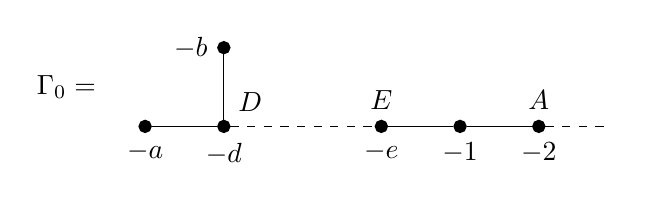
\begin{tikzpicture}
[bullet/.style={circle,draw=black!100,fill=black!100,thick,inner sep=0pt,minimum size=0.4em}]
\node (-105) at (-1,0.5) {$\Gamma_0=$};

\node[bullet] (00) at (0,0) [label=below:$-a$] {};
\node[bullet] (10) at (1,0) [label=below:$-d$, label=45:$D$] {};
\node[bullet] (11) at (1,1) [label=left:$-b$] {};
\node[bullet] (30) at (3,0) [label=below:$-e$, label=above:$E$] {};
\node[bullet] (40) at (4,0) [label=below:$-1$] {};
\node[bullet] (50) at (5,0) [label=below:$-2$, label=above:$A$] {};
\node (60) at (6,0) {};

\draw [-] (00) -- (10);
\draw [-] (10) -- (11);
\draw [dashed] (10) -- (30);
\draw [-] (30) -- (40);
\draw [-] (40) -- (50);
\draw [dashed] (50) -- (60);
\end{tikzpicture}
\end{center}
where $e \ge 3$. Note that the ($-e$)-vertex $E$ and the ($-d$)-vertex
$D$ (the node) may coincide.

If we blow down the ($-1$)-vertex of $\Gamma_0$ then the ($-2$)-vertex $A$ of $\Gamma_0$
becomes the ($-1$)-vertex of the new graph. Since a ($-1$)-vertex in a
star-shaped graph of ${\ensuremath \mathcal{A}}$, ${\ensuremath \mathcal{B}}$, or ${\ensuremath \mathcal{C}}$ with valencies $\le 3$ is
not a leaf, there must be a vertex attached to the right side of the
($-2$)-vertex $A$ of $\Gamma_0$. In summary, the non-minimal graph $\Gamma_1$
is of the form:
\begin{center}
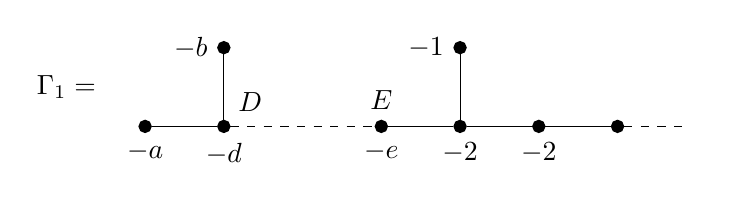
\begin{tikzpicture}
[bullet/.style={circle,draw=black!100,fill=black!100,thick,inner sep=0pt,minimum size=0.4em}]
\node (-105) at (-1,0.5) {$\Gamma_1=$};

\node[bullet] (00) at (0,0) [label=below:$-a$] {};
\node[bullet] (10) at (1,0) [label=below:$-d$, label=45:$D$] {};
\node[bullet] (11) at (1,1) [label=left:$-b$] {};
\node[bullet] (30) at (3,0) [label=below:$-e$, label=above:$E$] {};
\node[bullet] (40) at (4,0) [label=below:$-2$] {};
\node[bullet] (41) at (4,1) [label=left:$-1$] {};
\node[bullet] (50) at (5,0) [label=below:$-2$] {};
\node[bullet] (60) at (6,0) {};
\node (70) at (7,0) {};

\draw [-] (00) -- (10);
\draw [-] (10) -- (11);
\draw [dashed] (10) -- (30);
\draw [-] (30) -- (40);
\draw [-] (40) -- (50);
\draw [-] (40) -- (41);
\draw [-] (50) -- (60);
\draw [dashed] (60) -- (70);
\end{tikzpicture}
\end{center}
where $e \ge 3$. If $E=D$, then the minimal graph
$\overline{\Gamma}_1$ is of type $L_1-J_1-R_8$ using the contraction
$C_4$. If $E \neq D$, the graph
$\overline{\Gamma}_1$ is of type $L_1-J_1-R_8$ for $d \ge 3$ or
$L_2-J_1-R_8$ for $d=2$, concluding the argument in this subcase.

\textbf{Case 2:} Suppose now that the ($-2$)-vertex of $\Gamma_0$ is
to the left of the ($-1$)-vertex. Then the non-minimal graph
$\Gamma_1$ is given as follows:
\begin{center}
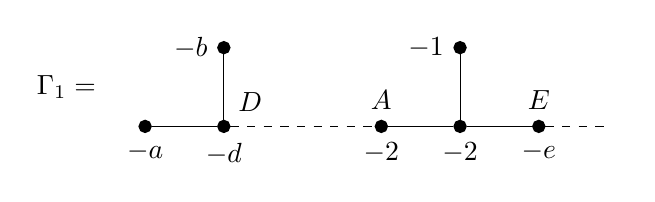
\begin{tikzpicture}
[bullet/.style={circle,draw=black!100,fill=black!100,thick,inner sep=0pt,minimum size=0.4em}]
\node (-105) at (-1,0.5) {$\Gamma_1=$};

\node[bullet] (00) at (0,0) [label=below:$-a$] {};
\node[bullet] (10) at (1,0) [label=below:$-d$, label=45:$D$] {};
\node[bullet] (11) at (1,1) [label=left:$-b$] {};
\node[bullet] (30) at (3,0) [label=below:$-2$, label=above:$A$] {};
\node[bullet] (40) at (4,0) [label=below:$-2$] {};
\node[bullet] (41) at (4,1) [label=left:$-1$] {};
\node[bullet] (50) at (5,0) [label=below:$-e$, label=above:$E$] {};
\node (60) at (6,0) {};

\draw [-] (00) -- (10);
\draw [-] (10) -- (11);
\draw [dashed] (10) -- (30);
\draw [-] (30) -- (40);
\draw [-] (40) -- (50);
\draw [-] (40) -- (41);
\draw [dashed] (50) -- (60);
\end{tikzpicture}
\end{center}
where $e \ge 3$. If $D=A$, then the minimal graph
$\overline{\Gamma}_1$ is of type $L_2-J_1-R_2$. Suppose that $D \neq
A$. If there is a ($-d$)-vertex with $d \ge 3$ between $D$ and $A$,
then $\overline{\Gamma}_1$ is of type $L_1-J_2-R_3$ for $d \ge 3$,
and, of type $L_2-J_2-R_3$ for $d=2$. Assume that there is no
($-d$)-vertex with $d \ge 3$ between $D$ and $A$. If $d \ge 3$, then
$\overline{\Gamma}_1$ is of type $L_1-J_2-R_3$ using the contraction
$C_3$. If $d=2$, then $E$ is a leaf of the graph and
$\overline{\Gamma}_1$ is of type $L_2-J_1-R_2$.
\end{proof}

\begin{remark}
J. Wahl informed us that
the example in~\cite[Remark~8.9]{Wahl-2011} was erroneously
claimed to be non-taut. The graph can be presented as $L_1-J_1-R_8$ using a contraction $C_4$ as we have seen above.
\end{remark}

We have a similar result for key-shaped graphs.

\begin{lemma}\label{lemma:key-shaped}
Let $\Gamma_1$ be a non-minimal key-shaped graph of type ${\ensuremath \mathcal{A}}$,
${\ensuremath \mathcal{B}}$, or ${\ensuremath \mathcal{C}}$ given by:
\begin{enumerate}

\item[(a)] \hfill

\begin{tikzpicture}
[bullet/.style={circle,draw=black!100,fill=black!100,thick,inner
    sep=0pt,minimum size=0.4em}] \node (-105) at (-1,0.5)
{$\Gamma_1=$};

\node[bullet] (00) at (0,0) [label=below:$-a$] {};
\node[bullet] (10) at (1,0) [label=315:$-d$] {};
\node[bullet] (11) at (1,1) [label=left:$-b$] {};
\node[bullet] (1-1) at (1,-1) [label=left:$-c$] {};
\node[bullet] (40) at (4,0) [label=below:$-e$] {};
\node[bullet] (41) at (4,1) [label=left:$-1$] {};
\node[bullet] (42) at (4,2) {};
\node[bullet] (60) at (6,0) {};

\draw [-] (00) -- (10);
\draw [-] (10) -- (11);
\draw [-] (10) -- (1-1);
\draw [dashed] (10) -- (40);
\draw [dashed] (40) -- (60);
\draw [dashed] (40) -- (41);
\draw [dashed] (41) -- (42);
\end{tikzpicture}

for $e \ge 3$; or

\item[(b)] \hfill

\begin{tikzpicture}
[bullet/.style={circle,draw=black!100,fill=black!100,thick,inner
    sep=0pt,minimum size=0.4em}] \node (-105) at (-1,0.5)
{$\Gamma_1=$};

\node[bullet] (00) at (0,0) [label=below:$-a$] {};
\node[bullet] (10) at (1,0) [label=315:$-d$] {};
\node[bullet] (11) at (1,1) [label=left:$-b$] {};
\node[bullet] (1-1) at (1,-1) [label=left:$-c$] {};
\node[bullet] (40) at (4,0) [label=below:$-2$] {};
\node[bullet] (41) at (4,1) [label=left:$-1$] {};
\node[bullet] (60) at (6,0) {};

\draw [-] (00) -- (10);
\draw [-] (10) -- (11);
\draw [-] (10) -- (1-1);
\draw [dashed] (10) -- (40);
\draw [dashed] (40) -- (60);
\draw [-] (40) -- (41);
\end{tikzpicture}
\end{enumerate}
where $(a, b, c)$ is one of the triples $(3, 3, 3)$, $(2, 4, 4)$, $(2,
3, 6)$ and $d \ge 3$. Let $\overline{\Gamma}_1$ be the corresponding minimal
graph. Then we have
\[h^1(S_{\overline{\Gamma}_1}, \Theta_{S_{\overline{\Gamma}_1}}(-\log{Z_{\overline{\Gamma}_1}}))=1.\]
\end{lemma}

\begin{proof}
Suppose that the analytic structure of the singularity
$X_{\overline{\Gamma}_1}$ (obtained by contracting
$Z_{\overline{\Gamma}_1}$ in $S_{\overline{\Gamma}_1}$) is determined
by the graph $\overline{\Gamma}_1$ and the analytic structure on the
reduced exceptional set $Z_{\overline{\Gamma}_1}$. By
Laufer~\cite[Theorem~3.2]{Laufer-1973-Taut} and
Laufer~\cite[(4.1)]{Laufer-1973-Taut}, a necessary and sufficient
condition for $\overline{\Gamma}_1$ and $Z_{\overline{\Gamma}_1}$ to
determine the singularity $X_{\overline{\Gamma}_1}$ is that the
restriction map
\begin{equation*}
H^1(Z_{\overline{\Gamma}_1}(s), \Theta_{Z_{\overline{\Gamma}_1}(s)}) \to H^1(Z_{\overline{\Gamma}_1}, \Theta_{Z_{\overline{\Gamma}_1}})
\end{equation*}
is an isomorphism. Since the analytic structure on
$Z_{\overline{\Gamma}_1}$ is uniquely determined by the cross ratio of
the 4 intersection points on the ($-d$)-curve with valency $4$, we
have
\[h^1(Z_{\overline{\Gamma}_1}, \Theta_{Z_{\overline{\Gamma}_1}})=1.\]
Hence it follows by Lemma~\ref{lemma:W<-E>=TZ} that
\begin{equation*}
\begin{split}
h^1(S_{\overline{\Gamma}_1}, \Theta_{S_{\overline{\Gamma}_1}}(-\log{Z_{\overline{\Gamma}_1}})) &= h^1(Z_{\overline{\Gamma}_1}(s), \Theta_{Z_{\overline{\Gamma}_1}(s)})= h^1(Z_{\overline{\Gamma}_1}, \Theta_{Z_{\overline{\Gamma}_1}})=1.
\end{split}
\end{equation*}
Therefore it is enough to show that the analytic structure of the
singularity $X_{\overline{\Gamma}_1}$ is determined by
$\overline{\Gamma}_1$ and $Z_{\overline{\Gamma}_1}$. For this we will
use the list in Laufer~\cite[Theorem~4.1]{Laufer-1973-Taut} of all
dual graphs for singularities which are determined by the graph and
the analytic structure on the reduced exceptional set. The proof is
similar to that of Lemma~\ref{lemma:H-taut}.

In Case (a) the graph $\overline{\Gamma}_1$ is of type $L_1'-J_1-R_1$
for $d \ge 5$, of type $L_1''-J_1-R_1$ for $d=4$, and of type
$L_2'-J_1-R_1$ for $d=3$ in the list of
Laufer~\cite[Theorem~4.1]{Laufer-1973-Taut}.

For Case (b), as in the proof of Lemma~\ref{lemma:H-taut}, we have two
cases:

\textbf{Case 1:} $\Gamma_1$ is given as follows:
\begin{center}
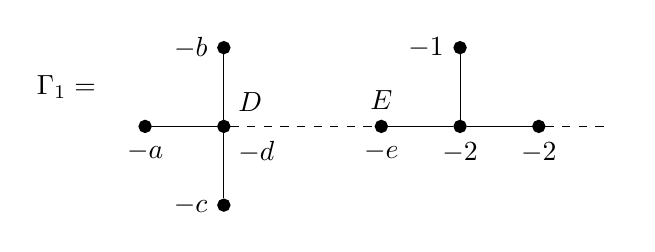
\begin{tikzpicture}
[bullet/.style={circle,draw=black!100,fill=black!100,thick,inner sep=0pt,minimum size=0.4em}]
\node (-105) at (-1,0.5) {$\Gamma_1=$};

\node[bullet] (00) at (0,0) [label=below:$-a$] {};
\node[bullet] (10) at (1,0) [label=315:$-d$, label=45:$D$] {};
\node[bullet] (11) at (1,1) [label=left:$-b$] {};
\node[bullet] (1-1) at (1,-1) [label=left:$-c$] {};
\node[bullet] (30) at (3,0) [label=below:$-e$, label=above:$E$] {};
\node[bullet] (40) at (4,0) [label=below:$-2$] {};
\node[bullet] (50) at (5,0) [label=below:$-2$] {};
\node[bullet] (41) at (4,1) [label=left:$-1$] {};
\node (60) at (6,0) {};

\draw [-] (00) -- (10);
\draw [-] (10) -- (11);
\draw [-] (10) -- (1-1);
\draw [dashed] (10) -- (30);
\draw [-] (30) -- (40);
\draw [-] (40) -- (50);
\draw [dashed] (50) -- (60);
\draw [-] (40) -- (41);
\end{tikzpicture}
\end{center}
where $e \ge 3$. Notice that since $d\geq 3$ (for $\overline{\Gamma}_1$ being a resolution graph of a rational surface singularity), the $(-1)$-framed vertex in a
star-shaped graph with valency 4 node and of type ${\ensuremath \mathcal{A}}, {\ensuremath \mathcal{B}}$, or ${\ensuremath \mathcal{C}}$
cannot be a leaf. For $d \ge 5$, $\overline{\Gamma}_1$ is of type
$L_1'-J_1-R_8$ possibly using the contraction $C_3$. For $d=4$, $\overline{\Gamma}_1$ is of type
$L_1''-J_1-R_8$ possibly using the contraction $C_4$. For $d=3$, if $D=E$ then $\overline{\Gamma}_1$ is of type $L_2'-J_1-R_2$, or if $D \neq E$ then $\overline{\Gamma}_1$ is of type $L_2'-J_1-R_8$.

\textbf{Case 2:} $\Gamma_1$ is given as follows:
\begin{center}
\begin{tikzpicture}
[bullet/.style={circle,draw=black!100,fill=black!100,thick,inner sep=0pt,minimum size=0.4em}]
\node (-105) at (-1,0.5) {$\Gamma_1=$};

\node[bullet] (00) at (0,0) [label=below:$-a$] {};
\node[bullet] (10) at (1,0) [label=315:$-d$] {};
\node[bullet] (11) at (1,1) [label=left:$-b$] {};
\node[bullet] (1-1) at (1,-1) [label=left:$-c$] {};
\node[bullet] (30) at (3,0) [label=below:$-2$] {};
\node[bullet] (40) at (4,0) [label=below:$-2$] {};
\node[bullet] (41) at (4,1) [label=left:$-1$] {};
\node[bullet] (50) at (5,0) [label=below:$-e$] {};
\node (60) at (6,0) {};

\draw [-] (00) -- (10);
\draw [-] (10) -- (11);
\draw [-] (10) -- (1-1);
\draw [dashed] (10) -- (30);
\draw [-] (30) -- (40);
\draw [-] (40) -- (50);
\draw [-] (40) -- (41);
\draw [dashed] (50) -- (60);
\end{tikzpicture}
\end{center}
where $e \ge 3$. For $d \ge 5$, $\overline{\Gamma}$ is of the form
$L_1'-J_2-R_3$ using the contraction $C_3$. For $d=4$, $\overline{\Gamma}$ is
of the form $L_1''-J_2-R_3$ using the contraction $C_3$. For $d=3$, $\overline{\Gamma}$ is of the form $L_2'-J_1-R_2$ if there are only ($-2$)-vertices between two nodes, or $\overline{\Gamma}$ is of the form $L_2'-J_2-R_3$ otherwise.
\end{proof}

\begin{lemma}\label{lemma:Gamma0}
Let $\Gamma_1$ be a non-minimal graph in Lemma~\ref{lemma:H-taut} or
Lemma~\ref{lemma:key-shaped}, and let $\Gamma_2$ be the non-minimal graph
obtained by blowing up once the ($-1$)-vertex of $\Gamma_1$. Then
\begin{equation*}
h^1(S_{\Gamma_2}, \Theta_{S_{\Gamma_2}}(-\log{Z_{\Gamma_2}})) = \alpha + \epsilon ,
\end{equation*}
where $\epsilon=0$ if $\Gamma_1$ is a graph in Lemma~\ref{lemma:H-taut},
$\epsilon=1$ if $\Gamma_1$ is a graph in Lemma~\ref{lemma:key-shaped}, and
$\alpha$ is given by Theorem~\ref{theorem:independent-alpha} (and it
depends only on the type of $\Gamma_1$).
\end{lemma}

\begin{proof}
It follows from Theorem~\ref{theorem:independent-alpha} that
\begin{equation*}
h^1(S_{\Gamma_1^{\sharp}}, \Theta_{S_{\Gamma_1^{\sharp}}}(-\log{Z_{\Gamma_1^{\sharp}}}))=\alpha + \epsilon.
\end{equation*}
Since $S_{\Gamma_1^{\sharp}}$ is obtained from $S_{\Gamma_2}$ by
blowing up edges emanating from the ($-1$)-curve (if needed), it follows by
Proposition~\ref{proposition:Flenner-Zaidenberg} that
\begin{equation*}
h^1(S_{\Gamma_2}, \Theta_{S_{\Gamma_2}}(-\log{Z_{\Gamma_2}}))=h^1(S_{\Gamma_1^{\sharp}}, \Theta_{S_{\Gamma_1^{\sharp}}}(-\log{Z_{\Gamma_1^{\sharp}}}))=\alpha + \epsilon. \qedhere
\end{equation*}
\end{proof}

\begin{theorem}\label{theorem:Technical-Main}
Let $\Gamma_1$ be a non-minimal graph in Lemma~\ref{lemma:H-taut} or
Lemma~\ref{lemma:key-shaped} and let $\Gamma_2$ be the non-minimal
graph obtained by blowing up once the ($-1$)-vertex of $\Gamma_1$. Let
$\Gamma$ be a non-minimal graph obtained from $\Gamma_2$ by applying
the blow-ups (B-1) and (B-2) (described in Section~\ref{sec:intro})
finitely many times. Suppose that $(X,0)$ is a rational surface
singularity with a resolution $(V,E)$ which admits the minimal graph
$\overline{\Gamma}$ as the resolution graph. Let $E=\sum_{i=1}^{n}
E_i$ be the decomposition of the exceptional divisor into
irreducible components $E_i$ with $E_i^2=-d_i$. Then
\[
h^1(V, \Theta_{V}(-\log{E})) + \sum_{i=1}^{n} (d_i-3)\leq 0.
\]
\end{theorem}

\begin{proof}
By Corollary~\ref{corollary:maximality} we have
\[h^1(V, \Theta_{V}(-\log{E})) \le
h^1(S_{\overline{\Gamma}},
\Theta_{S_{\overline{\Gamma}}}(-\log{Z_{\overline{\Gamma}}})).\]
Hence it is enough to show that
\begin{equation*}
h^1(S_{\overline{\Gamma}}, \Theta_{S_{\overline{\Gamma}}}(-\log{Z_{\overline{\Gamma}}})) + \sum_{i=1}^{n} (d_i-3) \le 0.
\end{equation*}

Let $m$ be the number of blow-ups of the ($-1$)-vertices to obtain the
non-minimal graph $\Gamma$ from $\Gamma_2$. Since $h^1(S_{\Gamma_2},
\Theta_{S_{\Gamma_2}}(-\log{Z_{\Gamma_2}})) = \alpha + \epsilon$ by
Lemma~\ref{lemma:Gamma0},
using Proposition~\ref{proposition:Flenner-Zaidenberg} it follows that
\begin{equation*}
h^1(S_{\Gamma}, \Theta_{S_{\Gamma}}(-\log{Z_{\Gamma}})) \le \alpha + \epsilon + m.
\end{equation*}
Then Theorem~\ref{theorem:independent-alpha}  implies that
\begin{equation}\label{equation:h1<=n}
h^1(S_{\overline{\Gamma}},
\Theta_{S_{\overline{\Gamma}}}(-\log{Z_{\overline{\Gamma}}})) \le \epsilon + m + 1.
\end{equation}

Note that for any minimal graph consisting of ($-e_i$)-vertices, the
blow-up procedure (B-1) with the modification (M) lowers the sum $\sum_{i=1}^{t} (e_i-3)$ by
$1$, while the procedure (B-2) with (M) leaves it unchanged; cf.\  the
proof of Wahl~\cite[Theorem~8.6]{Wahl-2011}. Since these sums for the
starting graphs $\overline{\Gamma}_{\ensuremath \mathcal{A}}$,
$\overline{\Gamma}_{\ensuremath \mathcal{B}}$, $\overline{\Gamma}_{\ensuremath \mathcal{C}}$ are equal to $1$,
this sum for $\overline{\Gamma}_2$ is $-\epsilon-1$. Since we blow up the ($-1$)-vertices $m$ times to obtain $\overline{\Gamma}$ from
$\overline{\Gamma}_2$, we have
\begin{equation}\label{equation:d-3}
\sum_{i=1}^{n} (d_i-3) = -\epsilon-1-m.
\end{equation}
From Equation~\eqref{equation:h1<=n} and Equation~\eqref{equation:d-3}
it follows that
\begin{equation*}
h^1(S_{\overline{\Gamma}},
\Theta_{S_{\overline{\Gamma}}}(-\log{Z_{\overline{\Gamma}}})) +
\sum_{i=1}^{n} (d_i-3) \le 0,
\end{equation*}
concluding the proof.
\end{proof}

Now we are in the position of giving the proof of Theorem~\ref{thm:nonexist},
which then implies the Main Theorem of the paper.

\begin{proof}[Proof of Theorem~\ref{thm:nonexist}]
Suppose first that $\overline{\Gamma}$ is of the form
$\overline{\Gamma}_1$ where $\Gamma_1$ is a non-minimal graph in
Lemma~\ref{lemma:H-taut} or Lemma~\ref{lemma:key-shaped}. If
$\Gamma_1$ is a non-minimal graph in Lemma~\ref{lemma:H-taut}, then we
have $h^1(S_{\overline{\Gamma}},
\Theta_{S_{\overline{\Gamma}}}(-\log{Z_{\overline{\Gamma}}})) =0$ by
Lemma~\ref{lemma:H-taut} and it is easy to see that $\sum_{i=1}^{n}
(d_i-3)=0$. Therefore, as in the proof of
Wahl~\cite[Theorem~8.6]{Wahl-2011}, we have
\begin{equation*}
h^1(S_{\overline{\Gamma}},
\Theta_{S_{\overline{\Gamma}}}(-\log{Z_{\overline{\Gamma}}})) +
\sum_{i=1}^{n} (d_i-3) = 0.
\end{equation*}
On the other hand, if $\Gamma_1$ is a non-minimal graph in Lemma~\ref{lemma:key-shaped}, then we have $h^1(S_{\overline{\Gamma}}, \Theta_{S_{\overline{\Gamma}}}(-\log{Z_{\overline{\Gamma}}})) = 1$ by Lemma~\ref{lemma:key-shaped}. But, since $\sum_{i=1}^{n} (d_i-3) = -1$, we have
\begin{equation*}
h^1(S_{\overline{\Gamma}}, \Theta_{S_{\overline{\Gamma}}}(-\log{Z_{\overline{\Gamma}}})) + \sum_{i=1}^{n} (d_i-3) = 0.
\end{equation*}

Suppose now that $\overline{\Gamma}$ is not of the form
$\overline{\Gamma}_1$ of Lemma~\ref{lemma:H-taut} or
Lemma~\ref{lemma:key-shaped}. Let $\Gamma_2$ be the non-minimal graph
obtained by blowing up the ($-1$)-vertex of $\Gamma_1$ once (as in
Theorem~\ref{theorem:Technical-Main}). Then $\overline{\Gamma}$ is
obtained by applying the blow-ups (B-1) and (B-2) to $\Gamma_2$
finitely many times, and finally the modification (M). The assertion
of the theorem now follows from Theorem~\ref{theorem:Technical-Main}.
\end{proof}

\begin{thebibliography}{99}
\bibitem{Bhupal-Stipsicz-2011} M.~Bhupal, A.~Stipsicz. \textit{Weighted
    homogeneous singularities and rational homology disk
    smoothings}. Amer.~J.~Math. \textbf{133} (2011), no.~5, 1259--1297.

\bibitem{Burns-Wahl-1974} D.~Burns, J.~Wahl. \textit{Local contributions to
    global deformations of surfaces}. Invent.~Math. \textbf{26} (1974),
  67--88.

\bibitem{deJong-VanStraten-1998} T.~de Jong, D.~van Straten. \textit{Deformation theory of sandwiched singularities}.  Duke Math J. \textbf{95} (1998),
  451--522.

\bibitem{Fintushel-Stern-1997} R.~Fintushel, R.~Stern. \textit{Rational
    blowdowns of smooth 4--manifolds}. J.~Differential Geom. \textbf{46}
  (1997), 181--235.

\bibitem{Flenner-Zaidenberg-1994} H.~Flenner,
  M. Zaidenberg. \textit{$\mathbb{Q}$-acyclic surfaces and their
    deformations}. Contemp.~Math. \textbf{162} (1994), 143--208.

\bibitem{Fowler-2013} J.~Fowler, \textit{Rational homology disk smoothing
    components of weighted-homogeneous surface singularities}. PhD Thesis, in
  preparation, 2013.

\bibitem{Grauert-1962} H.~Grauert, \textit{{\"U}ber Modifikationen und exzeptionelle analytische Mengen}. Math.~Ann. 146 (1962) 331--368.

\bibitem{Greuel-Steenbrink-1983} G.-M.~Greuel, J.~Steenbrink. \textit{On the
    topology of smoothable singularities}. Proc.~Sympos.~Pure Math. \textbf{40} (1983), 535--545.

\bibitem{Hartshorne-1977} R.~Hartshorne. \textit{Algebraic geometry}. Graduate Texts in Mathematics, no.~\textbf{52}. Springer-Verlag, 1977.

\bibitem{Keum-Lee-Park} J.~Keum, Y.~Lee, H.~Park. \textit{Construction of surfaces of general type from elliptic surfaces via $\mathbb{Q}$-Gorenstein smoothing}. Math.~Z. \textbf{272} (2012), no.~3--4, 1243--1257.

\bibitem{Kollar-Shepherd-Barron-1988} J.~Koll\'ar, N.~I.~Shepherd-Barron. \textit{Threefolds and deformations of surface singularities}. Invent.~Math. \textbf{91} (1988), no.~2, 299--338.

\bibitem{Laufer-1971} H.~Laufer. \textit{Normal two-dimensional singularities}. Annals of Mathematics Studies, no.~\textbf{71}. Princeton University Press, 1971.

\bibitem{Laufer-1973} H.~Laufer. \textit{Deformations of resolutions
  of two-dimensional singularities}. Complex analysis, 1972, Vol.~I:
  Geometry of singularities (Proc.~Conf., Rice Univ., Houston, Tex.,
  1972). Rice Univ.~Studies \textbf{59} (1973), no.~1, 53--96.

\bibitem{Laufer-1973-Taut} H.~Laufer. \textit{Taut two-dimensional singularities}. Math.~Ann. \textbf{205} (1973), 131--164.

\bibitem{Lee-Park-K^2=2} Y.~Lee, J.~Park. \textit{A simply connected surface of general type with $p_g=0$ and $K^2=2$}. Invent.~Math. \textbf{170} (2007), 483--505.

\bibitem{Looijenga-1984} E.~Looijenga. \textit{Isolated singular points on complete intersections}. London Mathematical Society Lecture Note Series \textbf{77}. Cambridge University Press, Cambridge, 1984.

\bibitem{Looijenga-Wahl-1986} E.~Looijenga, J.~Wahl. \textit{Quadratic functions and smoothing surface singularities}. Topology \textbf{25} (1986), no.~3, 261--291.

\bibitem{PPS-K3} H.~Park, J.~Park, D.~Shin. \textit{A simply connected surface of general type with $p_g=0$ and $K^2=3$}. Geom.~Topol. \textbf{13} (2009), no.~2, 743--767.

\bibitem{PPS-K4} H.~Park, J.~Park, D.~Shin. \textit{A simply connected surface of general type with $p_g=0$ and $K^2=4$}. Geom.~Topol. \textbf{13} (2009), no.~3, 1483--1494.

\bibitem{PPS-pg1} H.~Park, J.~Park, D.~Shin. \textit{Surfaces of general type with $p_g=1$ and $q=0$}. J.~Korean Math.~Soc. \textbf{50} (2013), no.~3,
493--507.

\bibitem{PPS-H1Z4} H.~Park, J.~Park, D.~Shin. \textit{A complex surface of general type with $p_g=0$, $K^2=2$ and $H_1=\mathbb{Z}/4\mathbb{Z}$}. Trans.~Amer.~Math.~Soc. \textbf{365} (2013), no.~11, 5713--5736.

\bibitem{PSU} H.~Park, D.~Shin, G.~Urz\'ua. \textit{A simply connected numerical Campedelli surface with an involution}. Math.~Ann. \textbf{357} (2013), no.~1, 31--49.

\bibitem{JPark-1997} J.~Park. \textit{Seiberg--Witten invariants of generalized rational blow--downs}. Bull.~Austral.~Math.~Soc. \textbf{56} (1997), 363--384.

\bibitem{JPark-2005} J. Park. \textit{Simply connected symplectic 4-manifolds with $b_2^+=1$ and $c_1^2=2$}. Invent.~Math. \textbf{159} (2005), no.~3, 657--667.

\bibitem{PSSz} J.~Park, A.~Stipsicz, Z.~Szab\'o. \textit{Exotic  smooth structures on ${\mathbb {CP}}^2 \# 5 {\overline {{\mathbb {CP}}^2}}$ }. Math.~Res.~Lett. \textbf{12} (2005), 701--712.

\bibitem{Schlessinger-1971} M.~Schlessinger. \textit{Rigidity of quotient singularities}. Invent.~Math. \textbf{14} (1971), 17--26.

\bibitem{Schuller-2012-thesis} F.~Sch\"uller. \textit{On taut singularities in arbitrary characteristics}. PhD thesis.

\bibitem{Schuller-2012} F.~Sch\"uller. \textit{On taut singularities
  in arbitrary characteristics}. arXiv:1303.6128.

\bibitem{SSz} A.~Stipsicz, Z.~Szab\'o. \textit{An exotic smooth
  structure on  ${\mathbb {CP}}^2 \# 6 {\overline {{\mathbb {CP}}^2}}$}.
Geom.~Topol. \textbf{9} (2005), 813--832.

\bibitem{Stipsicz-Szabo-Wahl-2008} A.~Stipsicz, Z.~Szab\'o, J.~Wahl. \textit{Rational blowdowns and smoothings of surface singularities}. J.~Topol. \textbf{1} (2008), no.~2, 477--517.

\bibitem{Wahl-1975} J.~Wahl. \textit{Vanishing theorems for resolutions of surface singularities}. Invent.~Math. \textbf{31} (1975), no.~1, 17--41.

\bibitem{Wahl-1981} J.~Wahl. \textit{Smoothings of normal surface singularities}. Topology \textbf{20} (1981), no.~3, 219--246.

\bibitem{Wahl-2011} J.~Wahl. \textit{On rational homology disk smoothings of valency 4 surface singularities}. Geom.~Topol. \textbf{15} (2011),  no.~2, 1125--1156.

\bibitem{Wahl-2011-log} J.~Wahl. \textit{Log-terminal smoothings of graded normal surface singularities}. Michigan Math. J. \textbf{62} (2013), no.~3, 475--489.

\bibitem{Wahl-2014} J.~Wahl. \textit{A personal commucation}.
\end{thebibliography}
\end{document}

